
\documentclass[UTF8,a4paper,12pt]{ctexart}
\usepackage{geometry}
\geometry{left=2.5cm,right=2.5cm,top=2.6cm,bottom=2.6cm}
\usepackage{amsmath,amssymb,bm}
\usepackage{booktabs,longtable,array,multirow}
\usepackage{graphicx}
\usepackage{float}
\usepackage{caption}
\usepackage{subcaption}
\usepackage{fancyhdr}
\usepackage{hyperref}
\usepackage{enumitem}
\usepackage{setspace}
\usepackage{titlesec}
\setstretch{1.25}
\setlength{\headheight}{15pt}
\pagestyle{fancy}
\fancyhf{}
\lhead{2011B 交巡警服务平台的设置与调度}
\rhead{数学建模论文}
\cfoot{\thepage}
\hypersetup{colorlinks=true,linkcolor=black,urlcolor=blue}
\graphicspath{{../figures/}}
\title{\heiti 基于路网最短路与覆盖优化的交巡警服务平台设置与调度模型}
\author{}
\date{}

\begin{document}
\maketitle

\begin{abstract}
交巡警服务平台兼具接处警、交通管理和社会服务功能，其设置与调度直接影响突发事件响应速度和重大事件封控效率。本文以某市主城六区交通网络、路口发案率、平台位置和出入口数据为基础，将道路抽象为带权无向图，采用 Dijkstra 最短路、最近服务分配、瓶颈匹配和贪心 $p$-中心改进模型，分别研究 A 区平台管辖、出入口封锁、新增平台选址、全市合理性评价和 P 点案发围堵方案。

针对问题一，本文首先以路网最短到达时间最小为准则，将 A 区 92 个节点分配给现有 20 个平台。结果显示，现状下 A 区仍有 6 个节点不能在 3 分钟内到达，最大到达时间为 5.70 min，平均到达时间为 1.12 min，平台工作量变异系数为 0.455。对 A 区 13 个出入口的快速封锁，采用最小化最大到达时间的二分阈值--匈牙利匹配模型，得到最大封锁到达时间 8.02 min、平均 3.55 min 的调度方案。

针对 A 区新增平台问题，本文在 2 至 5 个新增平台中逐一进行贪心选址比较。结果表明，新增 4 个平台即可使 A 区所有节点均满足 3 分钟响应要求，推荐位置为节点 28, 40, 48, 87；新增后最大到达时间降至 2.90 min，平均到达时间降至 0.88 min。新增第 5 个平台虽能进一步降低平均时间，但相对收益较小，故综合警力成本与覆盖效果选择新增 4 个平台。

针对问题二，本文从平台密度、人口负荷、发案负荷和 3 分钟覆盖率评价全市 80 个平台设置。现状下全市 582 个节点中有 138 个节点超过 3 分钟响应阈值，未覆盖率为 23.71\%，最大到达时间为 12.68 min；其中 F 区覆盖不足最突出，C 区单位平台发案负荷最高，说明现有设置存在明显不均衡。本文给出全市新增平台节点 517, 315, 408, 455, 206, 392, 509, 285, 239, 261 的改进建议，并保留原有平台体系。

针对 P 点（节点 32）重大刑事案件，本文考虑报警滞后 3 min，比较嫌疑人从 32 号节点到 17 个出入市区路口的剩余行驶时间和交巡警平台封锁到达时间。所给围堵方案对所有出口均能提前布控，最小安全裕度为 13.26 min，风险最高出口为节点 202。敏感性分析表明，在车速和时间阈值小幅扰动下，A 区新增平台数和全市薄弱区域判断保持稳定，模型具有较好的可复现性和解释性。

\textbf{关键词：}交巡警服务平台；最短路；覆盖优化；匈牙利算法；围堵调度
\end{abstract}

\newpage
\tableofcontents
\newpage

\section{问题重述}
\subsection{问题背景}
交巡警服务平台是城市警务系统中接近居民和道路交通节点的基层单元。平台数量过少会导致突发事件响应慢，平台数量过多又会造成警力资源浪费。因此，平台设置不是单纯的几何覆盖问题，而是同时涉及路网可达性、节点发案强度、辖区工作量均衡以及重大事件应急封控能力的综合优化问题。

本题给出了某市主城六区的路口坐标、道路连接、路口发案率、现有交巡警平台位置、出入城区路口以及各城区面积和人口数据。由于道路并非任意直线可通行，交巡警从平台到事发点的时间应基于道路网络最短路计算，而非简单欧氏距离。题目要求在现有平台基础上进行管辖范围划分、封锁调度、新增平台选址、全市设置合理性评价和刑事案件围堵调度。

\subsection{问题要求}
本文将题目拆分为五个相互关联的子任务：
\begin{enumerate}[label=\textbf{任务\arabic*：}]
  \item 对 A 区现有 20 个交巡警服务平台划分管辖范围，使所辖节点发生突发事件时尽量在 3 min 内到达。
  \item 对 A 区 13 个出入口进行重大突发事件全封锁调度，每个平台最多封锁一个路口。
  \item 在 A 区新增 2 至 5 个平台中选择合理数量和具体位置，以改善工作量不均衡和部分节点出警时间过长的问题。
  \item 面向全市六区评价现有平台设置是否合理，若不合理则提出改进方案。
  \item 对 P 点（节点 32）案发且报警滞后 3 min 的情形，给出全市平台围堵嫌疑车辆的调度方案。
\end{enumerate}

\section{问题分析}
\subsection{总体思路}
题目中的道路网络天然适合表示为图 $G=(V,E)$：节点代表交通路口，边代表道路，边权为两端路口坐标距离。题目给定地图距离与实际距离比例为 $1:100000$，即 1 mm 对应 100 m。警车时速为 60 km/h，即 1 km/min，因此道路距离 $d$ mm 对应时间 $0.1d$ min。基于该换算，3 min 响应阈值等价于 30 mm 的路网最短距离阈值。

整体建模流程为：首先读取并审计 Excel 数据，建立路网图；其次用 Dijkstra 算法计算平台到节点、平台到出入口和 P 点到出入口的最短路径距离；再次分别构建最近服务分配、瓶颈匹配、贪心选址和综合评价模型；最后将所有关键数字冻结，并据此生成论文图表和结论。

\subsection{各子问题方法选择}
对于管辖范围划分，最直接的 baseline 是按欧氏距离或路网最短时间分配最近平台。由于现实出警必须沿道路行驶，本文选择路网最短时间作为主模型，其输出能直接回答“哪个平台负责哪个节点”以及“是否 3 分钟可达”。

对于出入口封锁，任务本质是平台与出入口的一对一分配问题。若只按每个出口选择最近平台，可能同一平台被重复占用；若只最小化总时间，又可能存在个别出口封锁过慢。本文采用“先最小化最大到达时间，再兼顾总到达时间”的瓶颈匹配模型，既满足重大事件快速封锁的公平性，又保留整体效率。

对于新增平台选址，候选位置为 A 区路口节点。题目限定新增 2 至 5 个平台，属于离散设施选址问题。完全枚举组合数量较大，本文采用确定性贪心 $p$-中心改进：每一步选择使“3 分钟未覆盖节点数、最大到达时间、工作量变异系数”综合目标下降最多的节点。该方法可解释、可复现，且适合竞赛中快速得到稳定方案。

对于全市合理性评价，单一指标不足以说明设置合理性。本文从平台密度、人口负荷、发案负荷、平均到达时间、最大到达时间和 3 分钟未覆盖率六个维度评价，并提出改进节点。对于 P32 围堵，关键是报警滞后导致嫌疑人已行驶 3 min，因此必须比较“嫌疑人到出口剩余时间”和“平台到出口封锁时间”的安全裕度。

\section{数据来源、预处理与模型假设}
\subsection{数据来源与审计}
数据来自题目附件 2，共包含五个工作表：全市交通路口节点数据、全市交通路口路线、全市交巡警平台、全市区出入口位置和六城区基本数据。清洗后得到节点 582 个、道路边 928 条、交巡警平台 80 个、全市出入口 17 个、A 区出入口 13 个。节点坐标、所属区域和发案率均无缺失，平台位置无缺失，道路起终点无缺失；构造的无向交通网络连通，连通分量数为 1。

预处理步骤如下：
\begin{enumerate}[label=(\arabic*)]
  \item 仅保留各工作表的有效字段，删除说明列和空列；
  \item 将节点编号、道路端点和平台位置统一转为整数；
  \item 将坐标转为浮点数，将发案率缺失值视为 0；
  \item 以路口坐标欧氏距离作为道路边权，建立无向图；
  \item 按 $t=0.1d$ 将最短路距离换算为到达时间。
\end{enumerate}

\subsection{模型假设}
\begin{enumerate}[label=\textbf{假设\arabic*：}]
  \item 警车在道路上的平均速度为题目给定的 60 km/h。合理性：题目明确给出该速度；作用：用于将路网距离换算为到达时间。
  \item 突发事件发生后，最近负责平台可立即出警，不考虑警员上车、通信和道路拥堵造成的额外延迟。合理性：题目关注平台设置与调度，不提供拥堵数据；作用：使响应时间由路网最短时间决定。
  \item 道路为双向通行，边权等于两端节点坐标距离。合理性：附件道路图未给出单行线和道路等级；作用：建立无向加权图。
  \item 每个重大封锁任务中，一个平台最多封锁一个路口，且每个出入口需要一个平台。合理性：题目明确说明一个平台最多封锁一个路口；作用：构造一对一匹配模型。
  \item 新增平台只能设置在已有交通路口节点上。合理性：平台服务和出警需接入道路网络，且题目数据以路口为候选点；作用：将连续选址转化为离散选址。
\end{enumerate}

\section{符号说明}
\begin{table}[H]\centering
\caption{主要符号说明}
\begin{tabular}{cll}
\toprule
符号 & 含义 & 单位 \\
\midrule
$G=(V,E)$ & 城市交通网络图 & -- \\
$i,j$ & 交通路口节点编号 & -- \\
$p$ & 交巡警服务平台编号 & -- \\
$w_{ij}$ & 边 $(i,j)$ 的地图距离 & mm \\
$d(p,i)$ & 平台 $p$ 到节点 $i$ 的路网最短距离 & mm \\
$t(p,i)$ & 平台 $p$ 到节点 $i$ 的最短到达时间 & min \\
$r_i$ & 节点 $i$ 的日均发案率 & 次/日 \\
$x_{pi}$ & 节点 $i$ 是否由平台 $p$ 管辖 & 0/1 \\
$y_{pe}$ & 平台 $p$ 是否封锁出入口 $e$ & 0/1 \\
$T$ & 3分钟响应阈值 & min \\
\bottomrule
\end{tabular}
\end{table}

\section{模型建立与求解}
\subsection{路网最短路模型}
设道路边 $(i,j)$ 的坐标为 $(X_i,Y_i)$ 与 $(X_j,Y_j)$，则边权为
\begin{equation}
w_{ij}=\sqrt{(X_i-X_j)^2+(Y_i-Y_j)^2} .
\end{equation}
由于 1 mm 对应 0.1 km，警车速度为 1 km/min，因此平台 $p$ 到节点 $i$ 的到达时间为
\begin{equation}
t(p,i)=0.1\,d(p,i),
\end{equation}
其中 $d(p,i)$ 为图 $G$ 上以 $w_{ij}$ 为边权的最短路距离。本文对每个平台运行 Dijkstra 算法得到到所有节点或出入口的最短距离。

\subsection{问题一：A区平台管辖范围分配}
\subsubsection{模型建立}
本问要求为 A 区现有平台分配管辖节点。令 $P_A$ 为 A 区平台集合，$V_A$ 为 A 区节点集合。每个节点由到达时间最短的平台负责：
\begin{equation}
x_{pi}=\begin{cases}
1, & p=\arg\min_{q\in P_A} t(q,i),\\
0, & \text{其他情况}.
\end{cases}
\end{equation}
平台 $p$ 的工作量用其管辖节点发案率总和表示：
\begin{equation}
L_p=\sum_{i\in V_A} r_i x_{pi}.
\end{equation}
以 3 min 为响应阈值，未覆盖节点集合为
\begin{equation}
U=\{i\in V_A\mid \min_{p\in P_A}t(p,i)>3\}.
\end{equation}
该模型的 baseline 是欧氏最近平台分配；主模型改用路网最短时间，能够避免道路绕行导致的误判。

\subsubsection{求解结果与分析}
现有 A 区共有 92 个节点和 20 个平台。由路网最短路分配得到，A 区现状下有 6 个节点超过 3 min 阈值，占 6.52\%；最大到达时间 5.70 min，平均到达时间 1.12 min。平台工作量最大的平台为 A20，日均发案率负荷 11.50，最小平台负荷为 1.60，变异系数 0.455，说明现有管辖若完全按最近平台划分，部分平台负荷明显偏高。

\begin{figure}[H]\centering
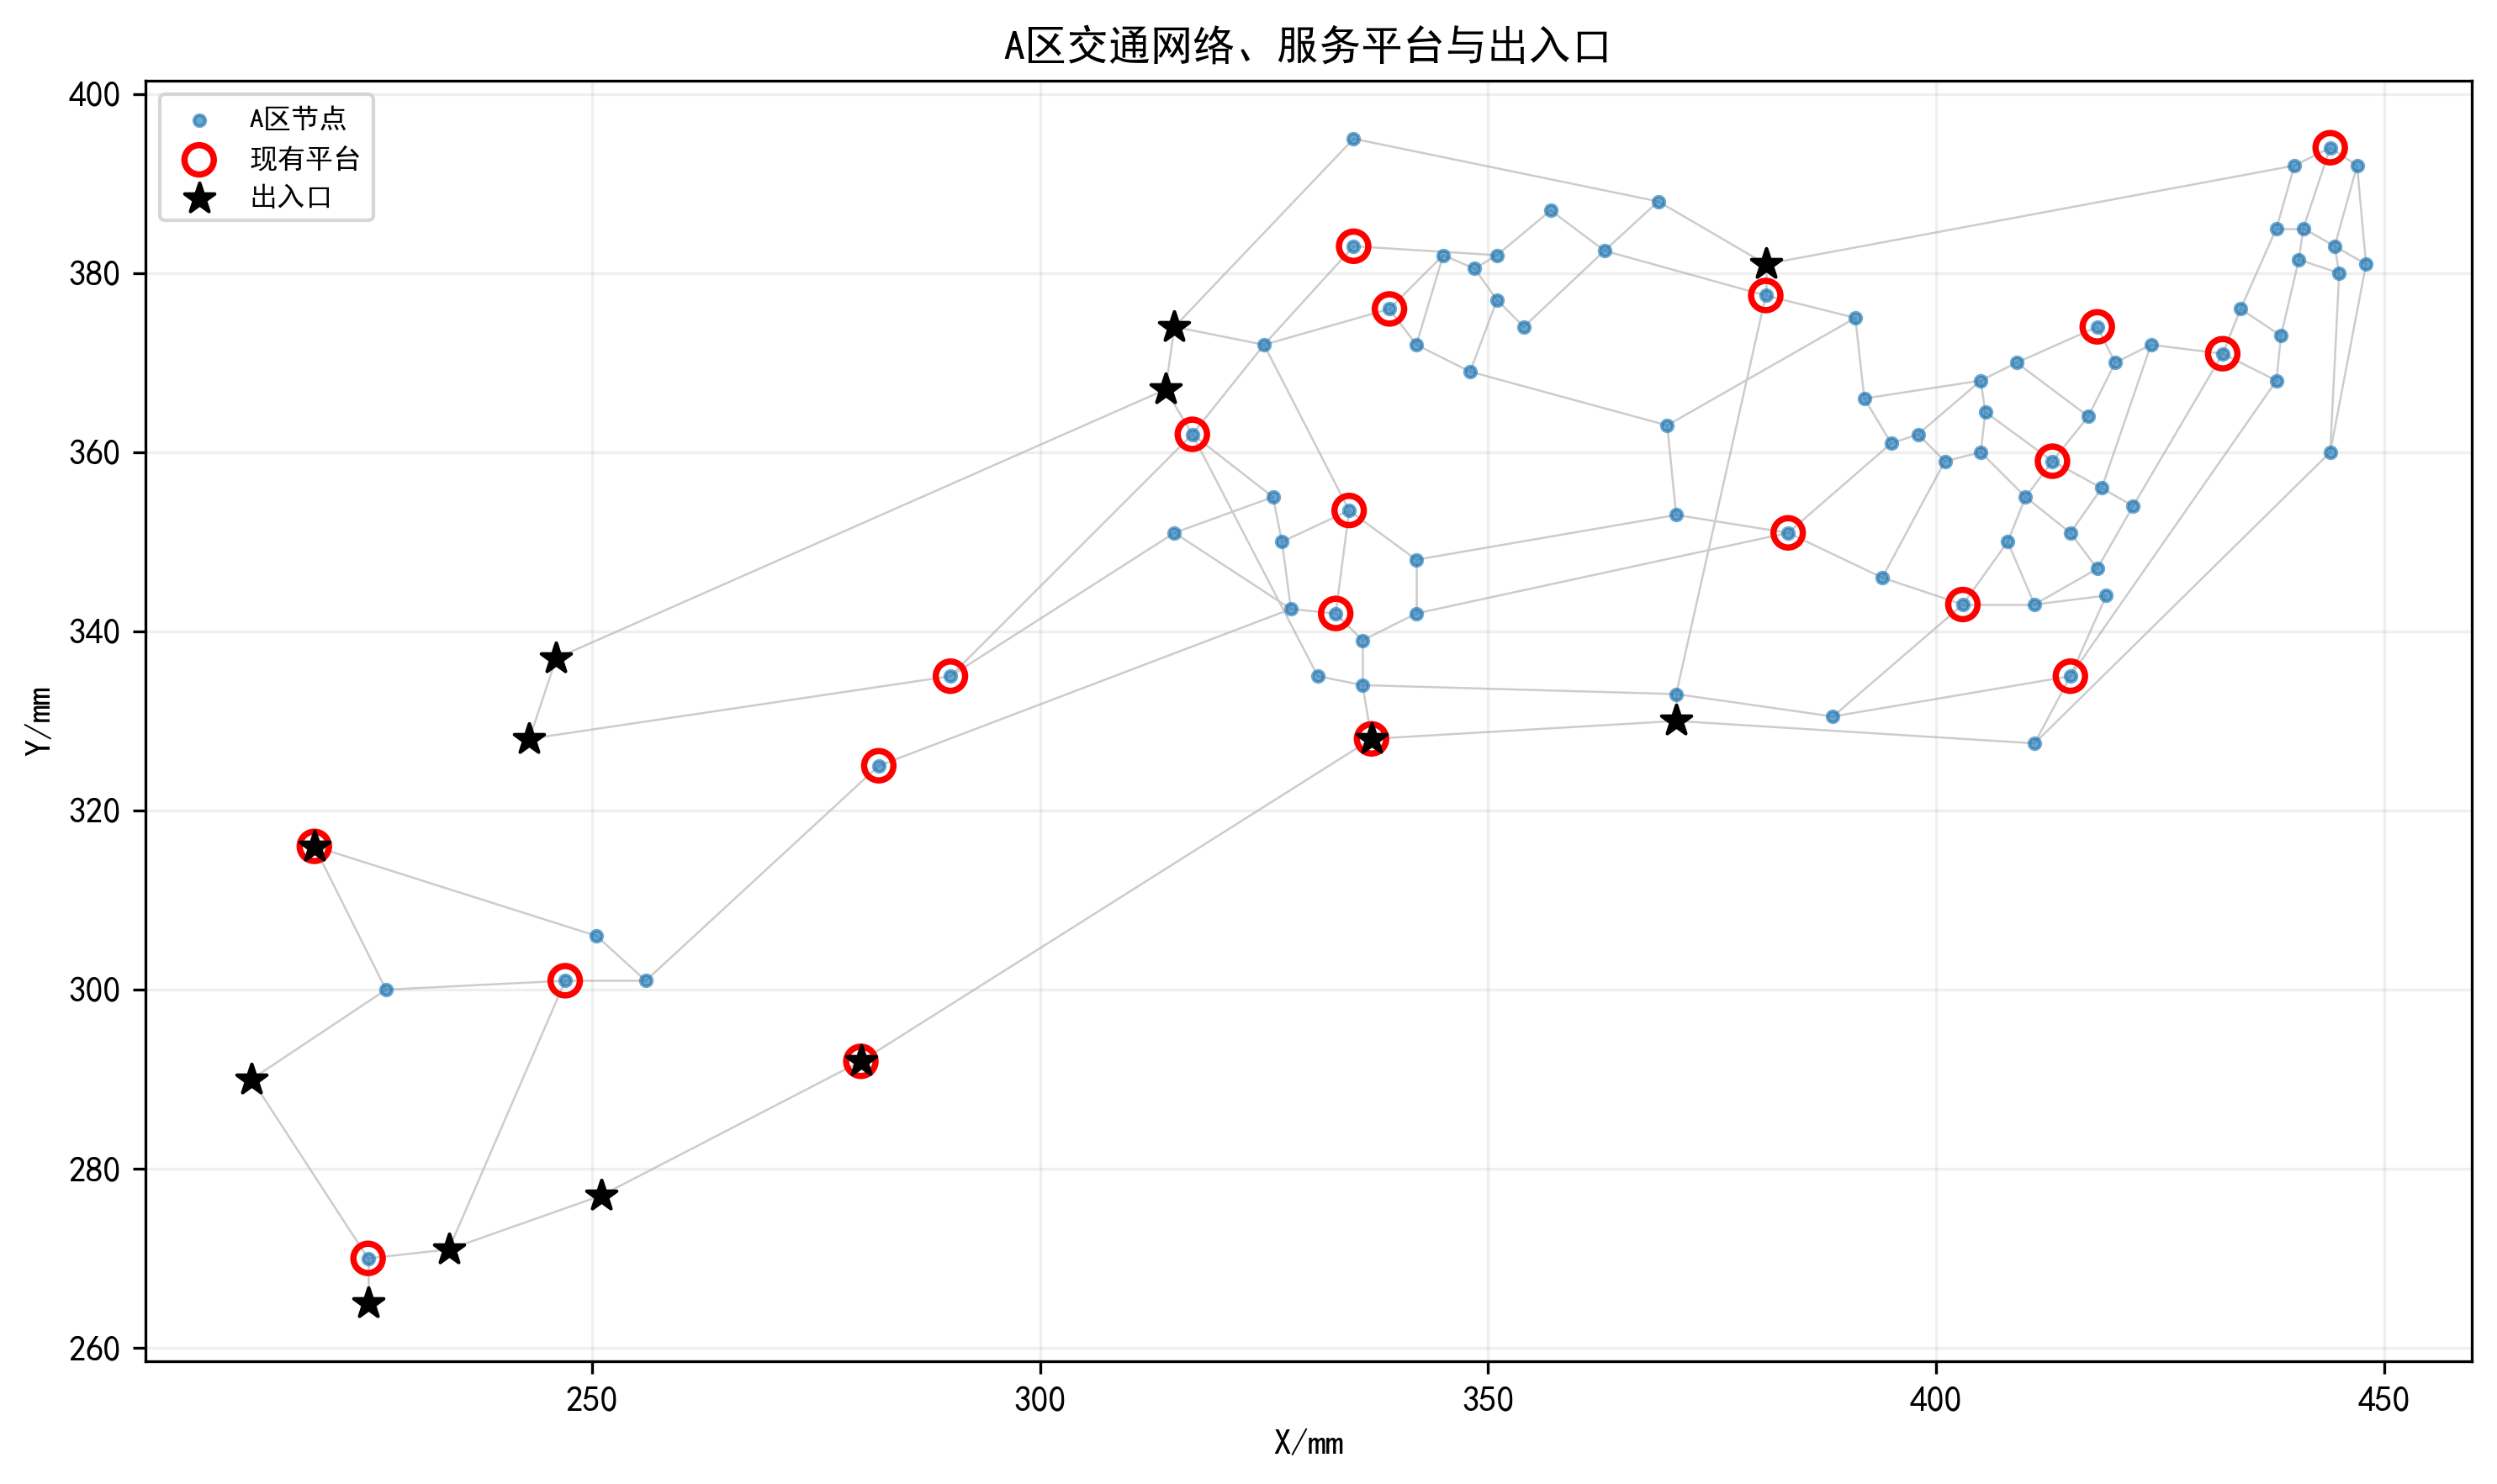
\includegraphics[width=0.82\textwidth]{问题1_A区网络平台与出入口.png}
\caption{A区交通网络、服务平台与出入口}
\end{figure}
图中红色空心圆表示现有平台，黑色星号表示 A 区出入口。可以看出平台集中分布于 A 区内部主干路附近，边缘若干节点与最近平台之间存在较长道路路径，这是少数节点超过 3 min 的主要原因。

\begin{figure}[H]\centering
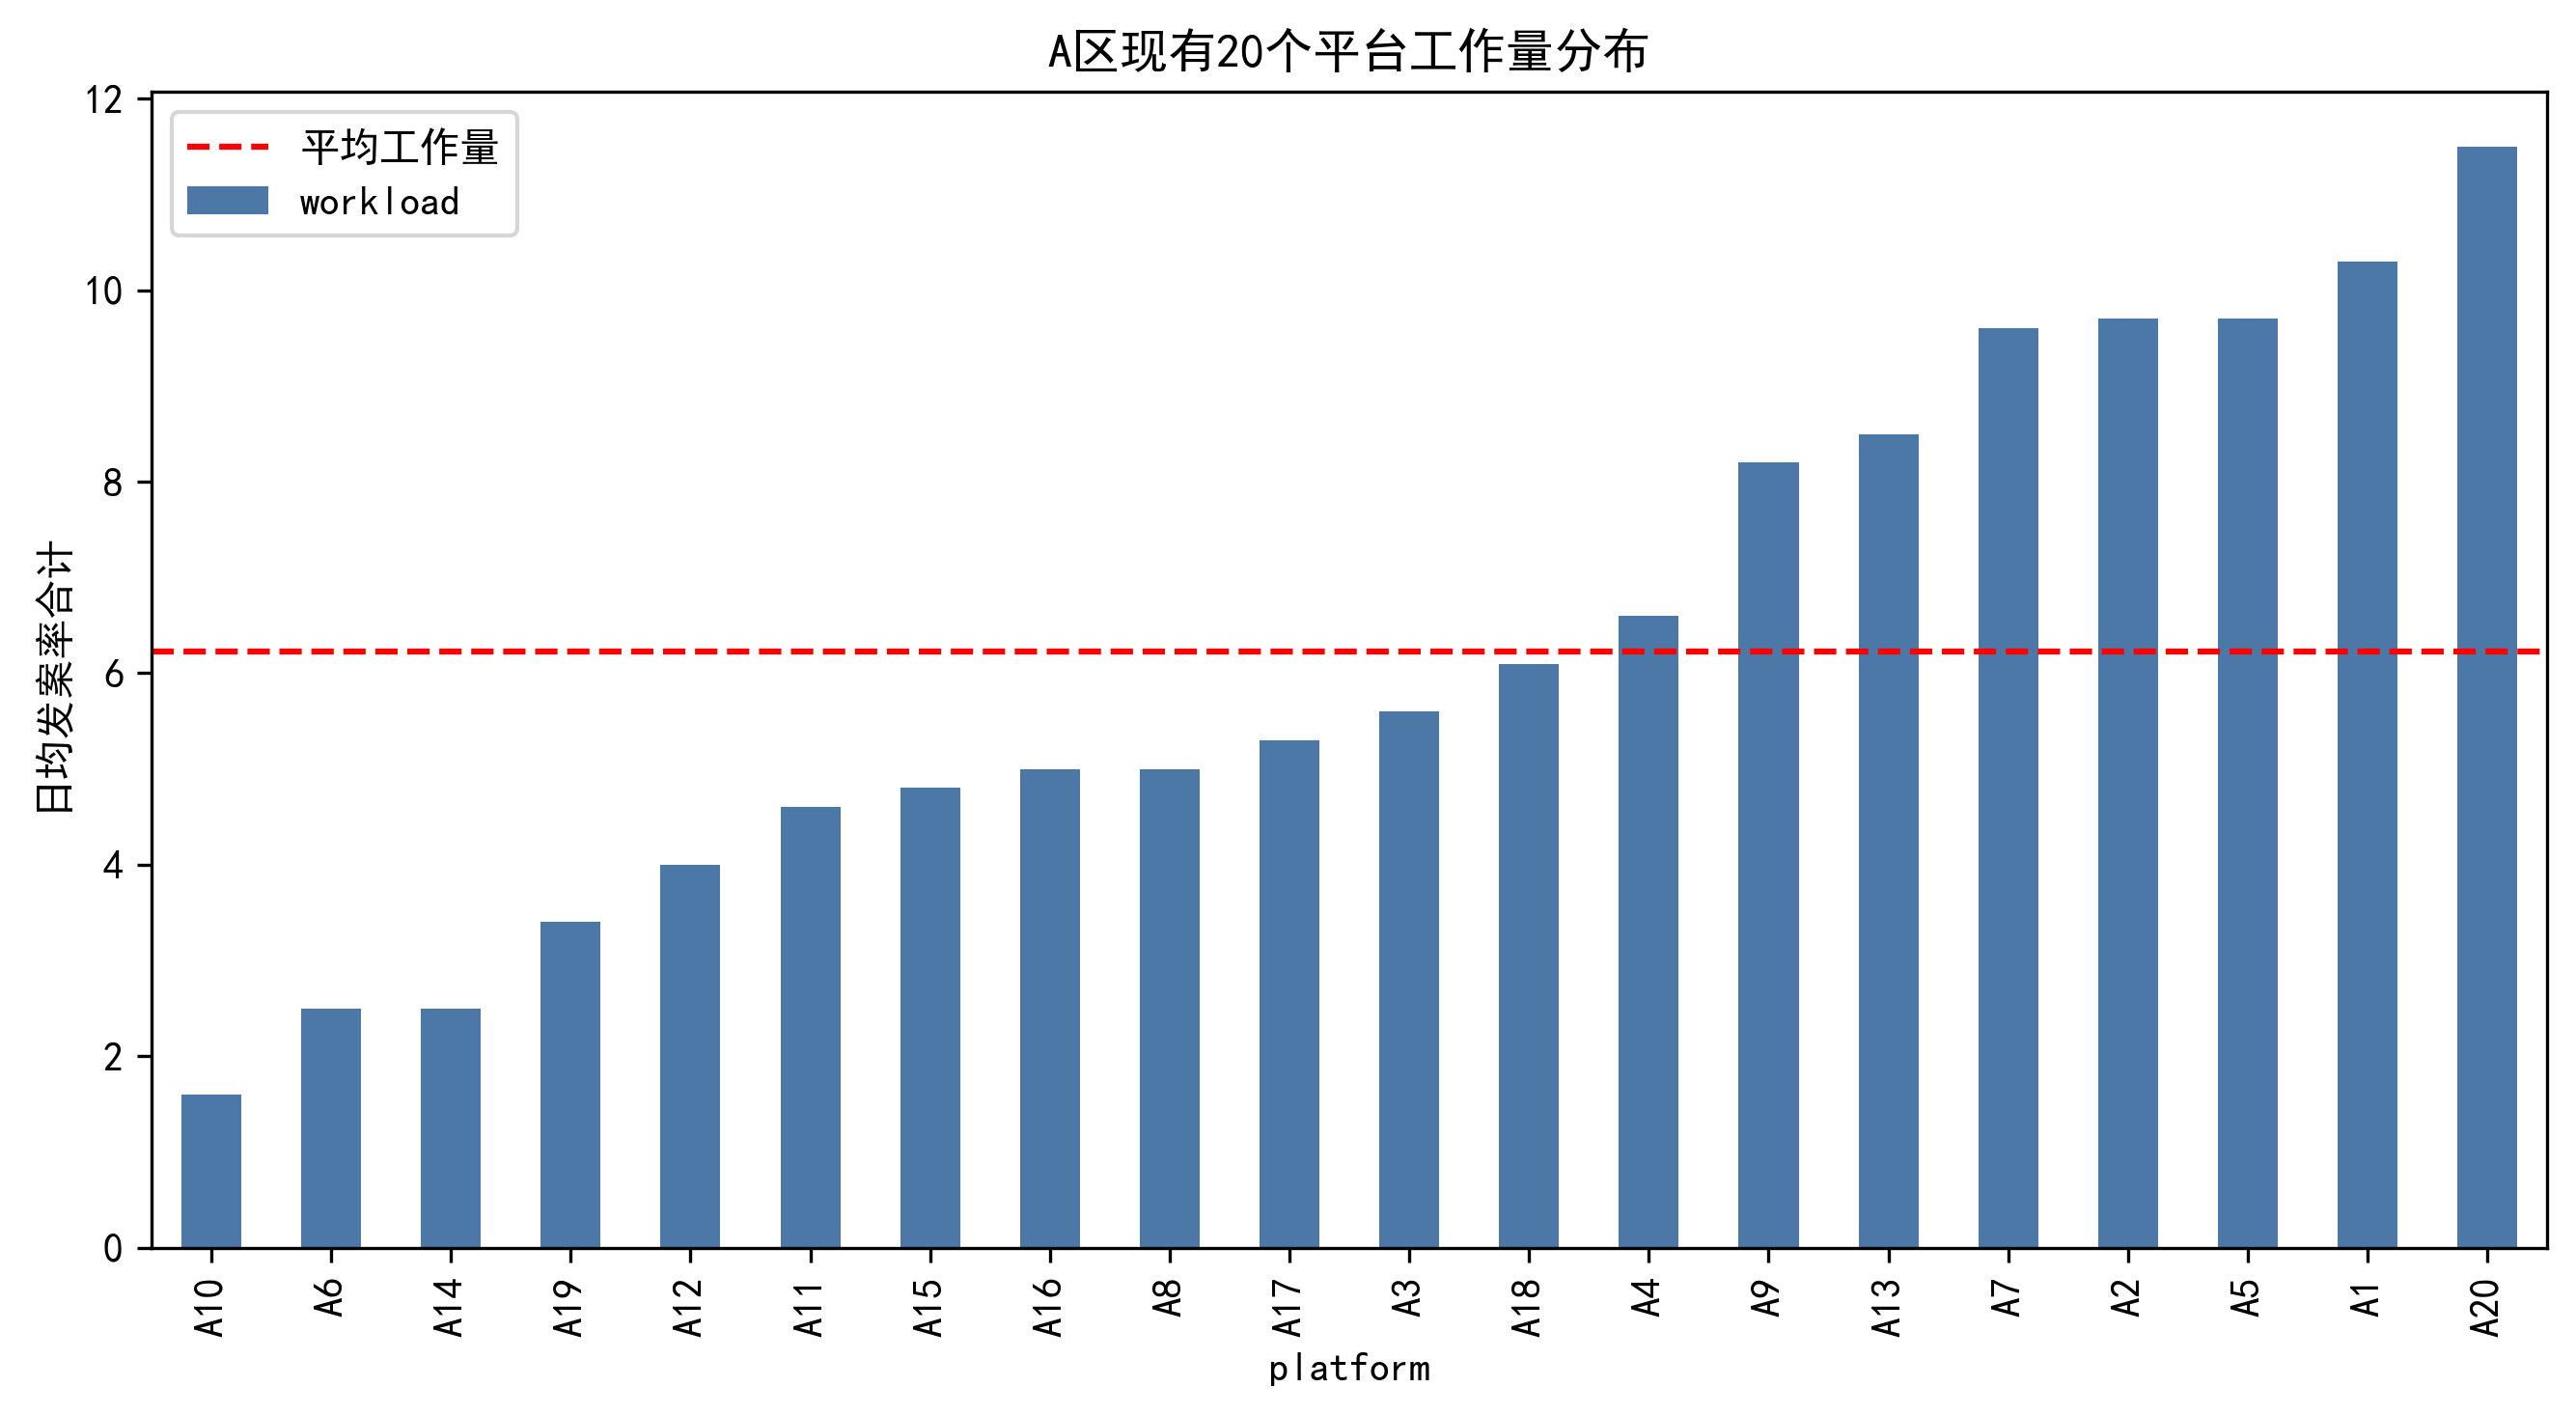
\includegraphics[width=0.82\textwidth]{问题1_A区现有平台工作量.png}
\caption{A区现有平台工作量分布}
\end{figure}
图中虚线为平均工作量。A20 等平台管辖节点发案率较高，而部分平台负荷明显低于平均值，说明仅依赖现有平台和最近分配规则会产生工作量不均衡。

\subsection{问题一：A区13个出入口封锁调度}
\subsubsection{模型建立}
设 A 区出入口集合为 $E_A$。决策变量 $y_{pe}$ 表示平台 $p$ 是否负责封锁出入口 $e$。考虑重大事件中最慢封锁点决定全封锁完成时间，建立瓶颈匹配模型：
\begin{align}
\min \quad & Z=\max_{p\in P_A,e\in E_A} t(p,e)y_{pe},\\
\text{s.t.}\quad & \sum_{p\in P_A} y_{pe}=1,\quad \forall e\in E_A,\\
& \sum_{e\in E_A} y_{pe}\le 1,\quad \forall p\in P_A,\\
& y_{pe}\in\{0,1\}.
\end{align}
求解时对候选阈值 $Z$ 二分/枚举，判断在 $t(p,e)\le Z$ 的二部图中是否存在覆盖所有出入口的匹配；在最小可行阈值内，再用匈牙利算法最小化总到达时间。

\subsubsection{调度方案}
\begin{table}[H]\centering
\caption{A区13个出入口封锁调度方案}
\begin{tabular}{rrrr}
\toprule
A区出口 & 调度平台 & 平台节点 & 到达/min \\
\midrule
12 & A12 & 12 & 0.000 \\
14 & A16 & 16 & 6.742 \\
16 & A9 & 9 & 1.533 \\
21 & A14 & 14 & 3.265 \\
22 & A10 & 10 & 7.708 \\
23 & A13 & 13 & 0.500 \\
24 & A11 & 11 & 3.805 \\
28 & A15 & 15 & 4.752 \\
29 & A7 & 7 & 8.015 \\
30 & A8 & 8 & 3.061 \\
38 & A2 & 2 & 3.982 \\
48 & A5 & 5 & 2.476 \\
62 & A4 & 4 & 0.350 \\
\bottomrule
\end{tabular}
\end{table}
方案最大到达时间为 8.02 min，平均到达时间为 3.55 min。由于部分出入口远离现有平台，单靠现有 20 个平台无法使所有出入口都在 3 min 内完成封锁，但该方案已在“一平台最多封锁一个路口”的约束下最小化了最慢封锁时间。

\subsection{问题一：A区新增平台选址}
\subsubsection{模型建立}
新增平台候选集合为 $C=V_A\setminus P_A$。对给定新增数量 $k$，目标首先最小化 3 min 未覆盖节点数，其次最小化最大到达时间并改善工作量均衡。综合目标写为
\begin{equation}
F(S)=10000|U(S)|+100\max_{i\in V_A}\min_{p\in P_A\cup S}t(p,i)+10CV(L(S)),
\end{equation}
其中 $S\subset C, |S|=k$，$CV(L)$ 为平台工作量变异系数。大权重保证模型优先满足 3 min 覆盖，再考虑时间与均衡。本文对 $k=2,3,4,5$ 分别用贪心策略求解：每一步加入使 $F$ 下降最多的候选节点。

\subsubsection{结果比较}
\begin{table}[H]\centering
\caption{A区新增平台数量比较}
\begin{tabular}{r l r r r r}
\toprule
新增数 & 新增节点 & 未覆盖节点 & 最大到达/min & 平均到达/min & 负荷CV \\
\midrule
2 & 28,40 & 2 & 4.190 & 0.962 & 1.551 \\
3 & 28,40,48 & 1 & 3.601 & 0.932 & 1.577 \\
4 & 28,40,48,87 & 0 & 2.900 & 0.877 & 1.623 \\
5 & 28,40,48,87,61 & 0 & 2.708 & 0.845 & 1.666 \\
\bottomrule
\end{tabular}
\end{table}
由表可知，新增 2 个平台后仍有 2 个节点超过 3 min；新增 3 个平台后仍有 1 个节点超过 3 min；新增 4 个平台后未覆盖节点降为 0，最大到达时间为 2.90 min。新增 5 个平台虽进一步将最大时间降至 2.71 min，但边际改善小于新增平台成本。因此本文推荐新增 4 个平台，位置为节点 28, 40, 48, 87。

\begin{figure}[H]\centering
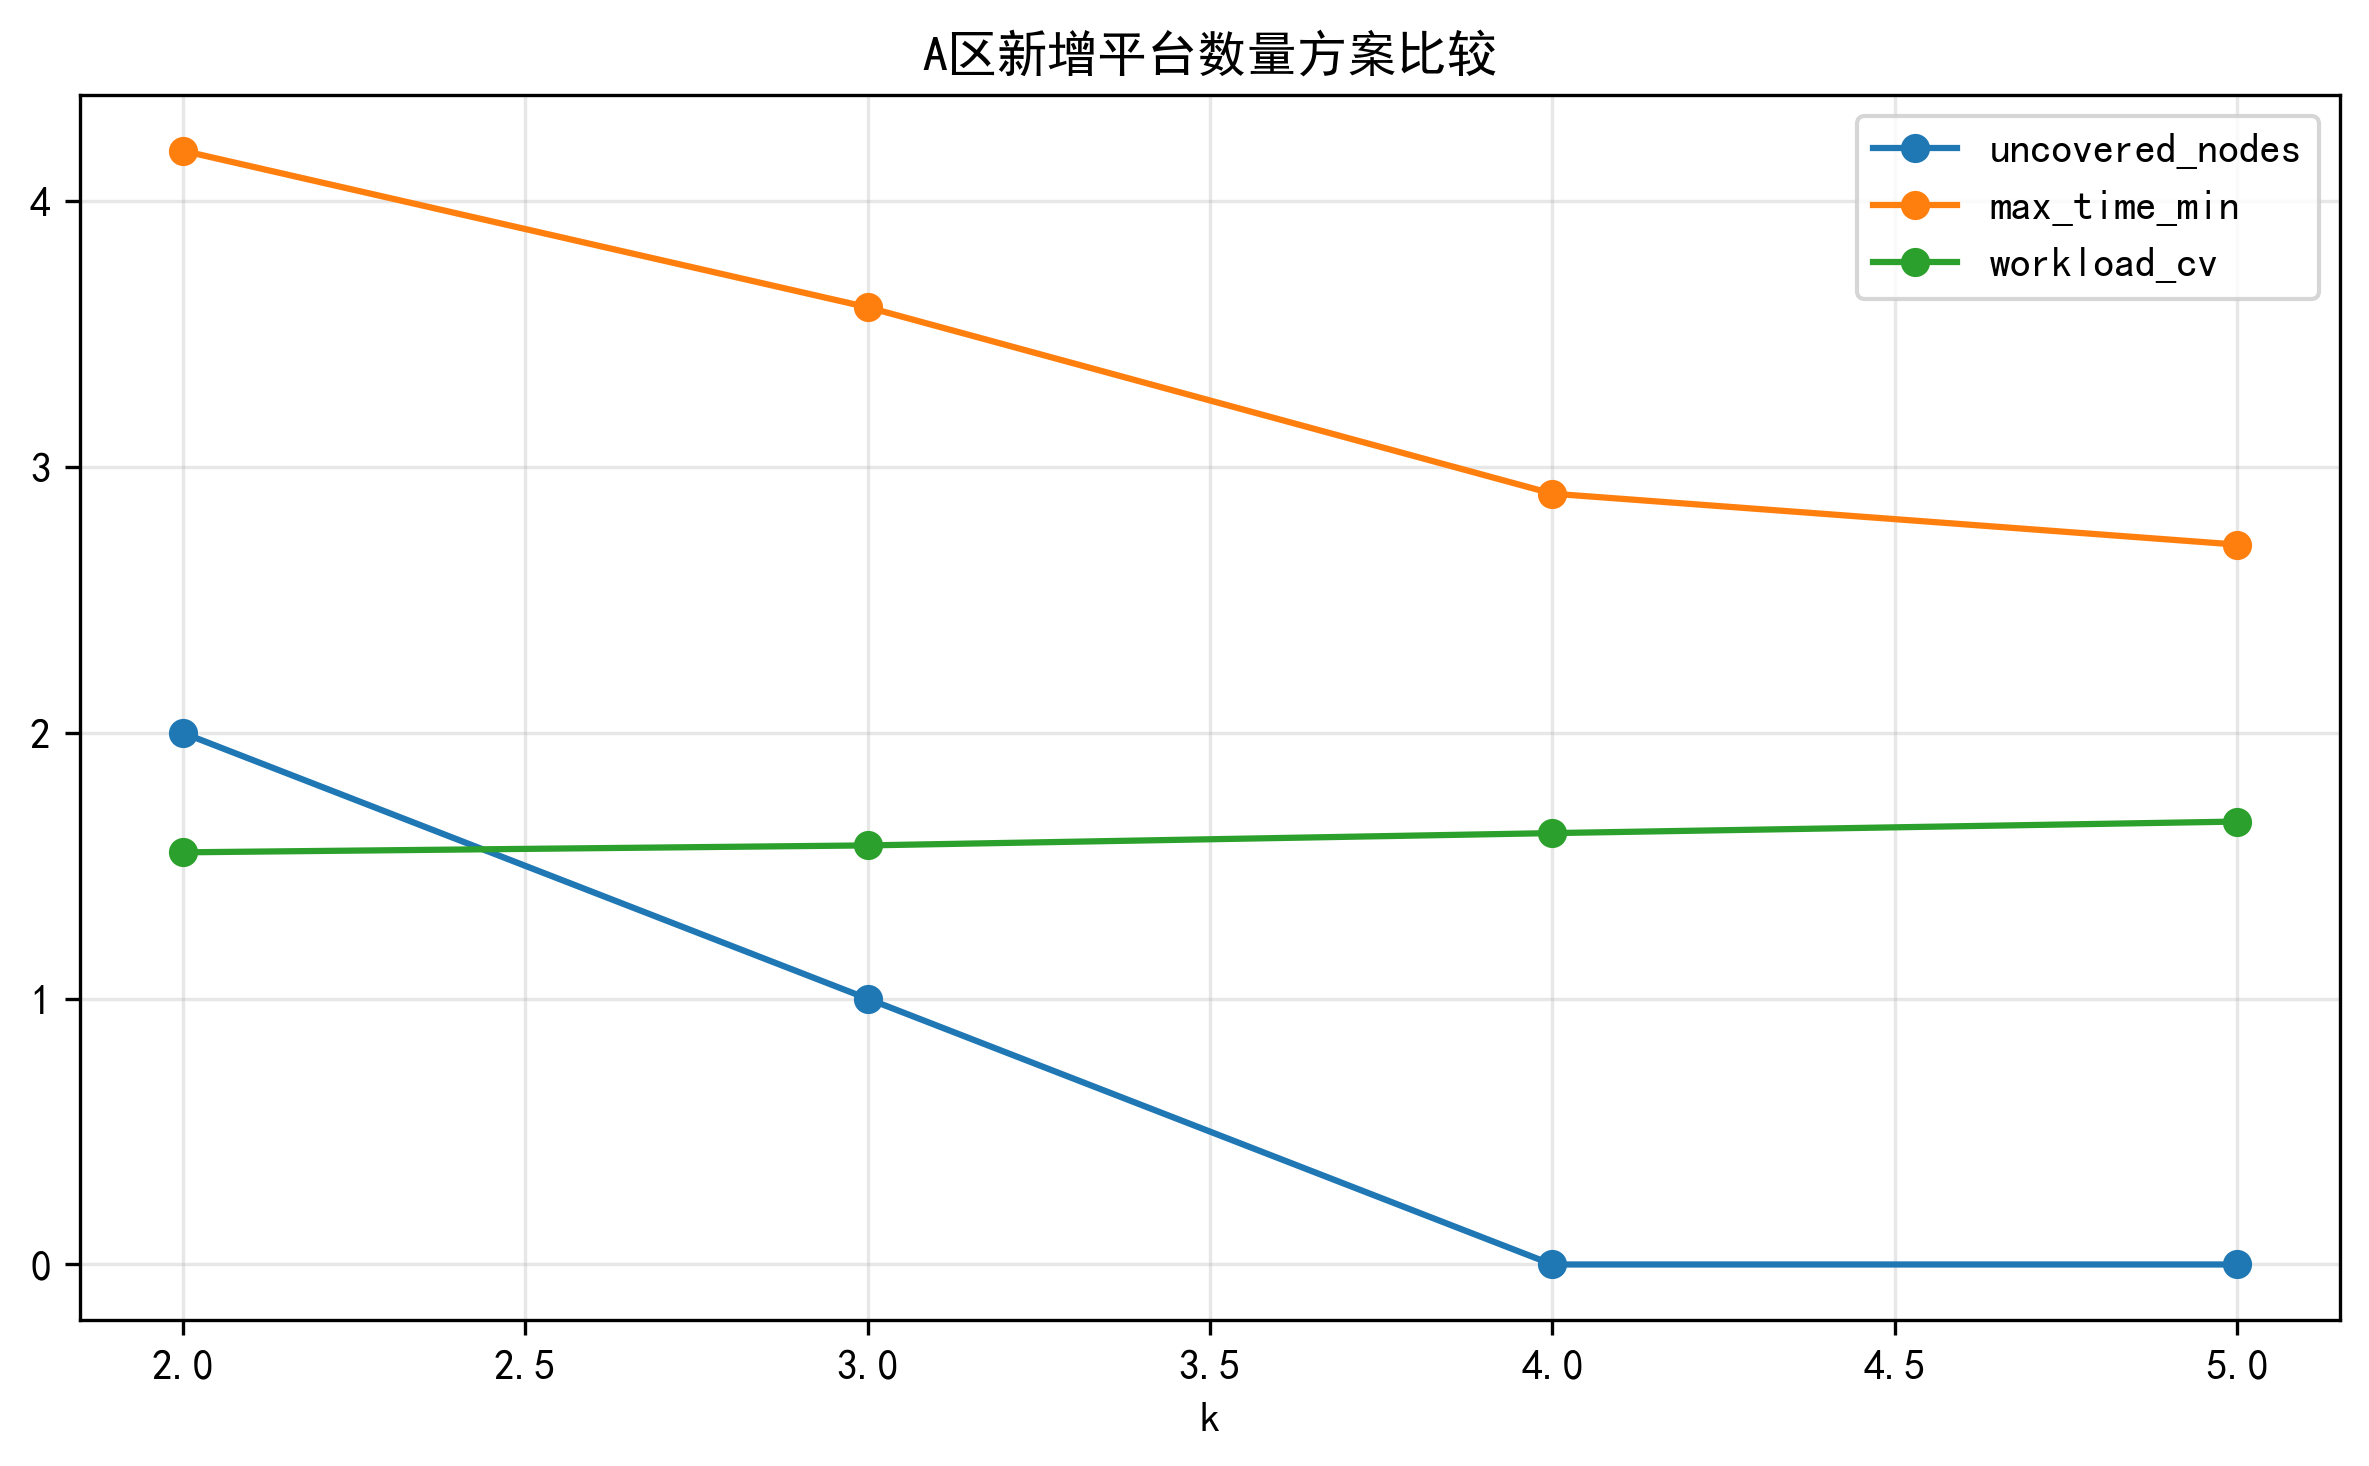
\includegraphics[width=0.82\textwidth]{问题1_新增平台数量比较.png}
\caption{A区新增平台数量方案比较}
\end{figure}
该图显示随着新增平台数量增加，未覆盖节点数和最大到达时间逐步下降。新增第 4 个平台是关键转折点，使 3 min 覆盖约束完全满足；新增第 5 个平台主要改善平均时间，已不是满足题目核心约束所必需。

\begin{figure}[H]\centering
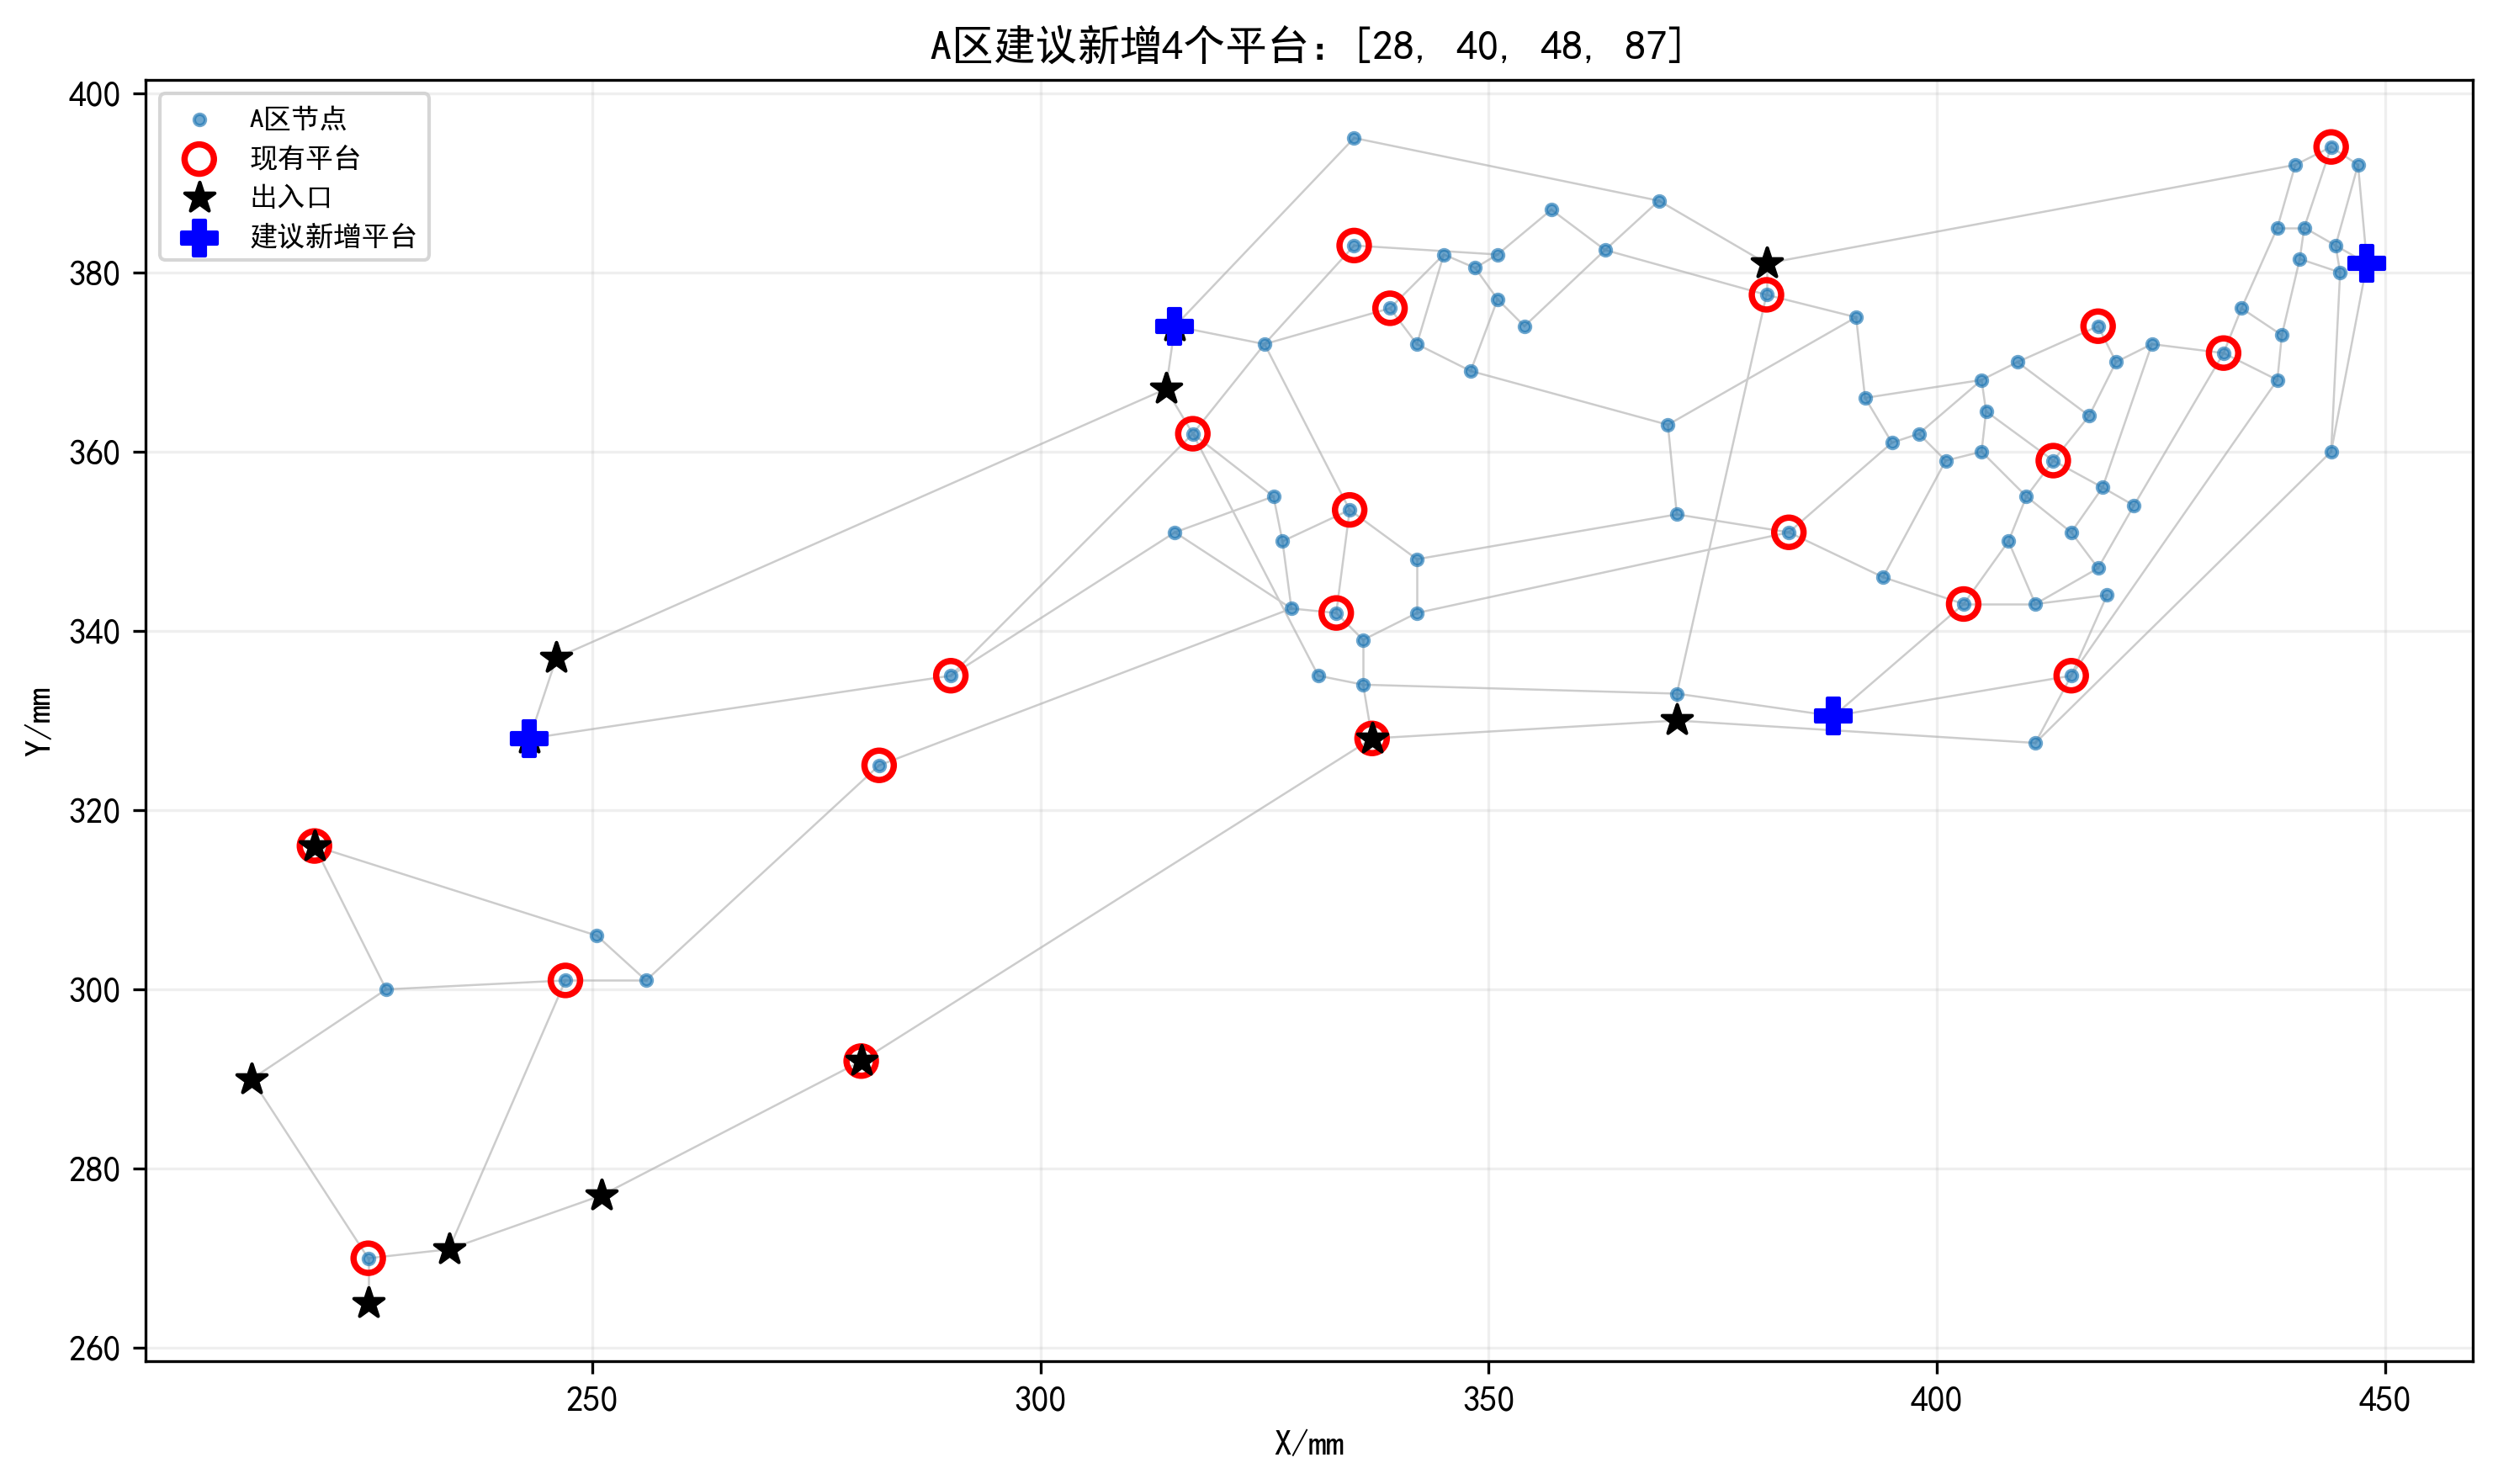
\includegraphics[width=0.82\textwidth]{问题1_A区建议新增平台.png}
\caption{A区建议新增平台位置}
\end{figure}
新增节点主要位于现有服务薄弱或边缘通达性不足的位置，能够补齐现有平台网络的覆盖空洞。

\subsection{问题二：全市平台设置合理性评价}
\subsubsection{评价指标}
全市评价既要考虑响应时间，又要考虑城区差异。本文设置以下指标：
\begin{enumerate}[label=(\arabic*)]
  \item 平台密度：每 $100\text{ km}^2$ 平台数，反映空间覆盖资源；
  \item 人口负荷：每万人平台数，反映服务人口压力；
  \item 发案负荷：每平台承担日均发案率，反映警务工作量；
  \item 平均到达时间和最大到达时间，反映响应效率；
  \item 3 min 未覆盖率，反映平台设置短板。
\end{enumerate}

\subsubsection{评价结果}
\begin{table}[H]\centering\small
\caption{全市六城区平台设置合理性评价}
\begin{tabular}{lrrrrrr}
\toprule
城区 & 平台数 & 节点数 & 发案率合计 & 未覆盖率 & 最大到达/min & 每平台发案率 \\
\midrule
A & 20 & 92 & 124.500 & 0.065 & 5.701 & 6.225 \\
B & 8 & 73 & 66.400 & 0.082 & 4.470 & 8.300 \\
C & 17 & 154 & 187.200 & 0.305 & 6.861 & 11.012 \\
D & 9 & 52 & 67.800 & 0.231 & 9.899 & 7.533 \\
E & 15 & 103 & 119.400 & 0.311 & 12.680 & 7.960 \\
F & 11 & 108 & 109.200 & 0.324 & 7.042 & 9.927 \\
\bottomrule
\end{tabular}
\end{table}
现状下，全市 582 个节点中有 138 个节点超过 3 min，未覆盖率 23.71\%，最大到达时间 12.68 min。从城区看，A 区平台密度最高，未覆盖率仅 6.52\%；而 F 区未覆盖率最高，达到 32.41\%。C 区每平台发案负荷最高，说明现有设置在工作量维度也不均衡。

\begin{figure}[H]\centering
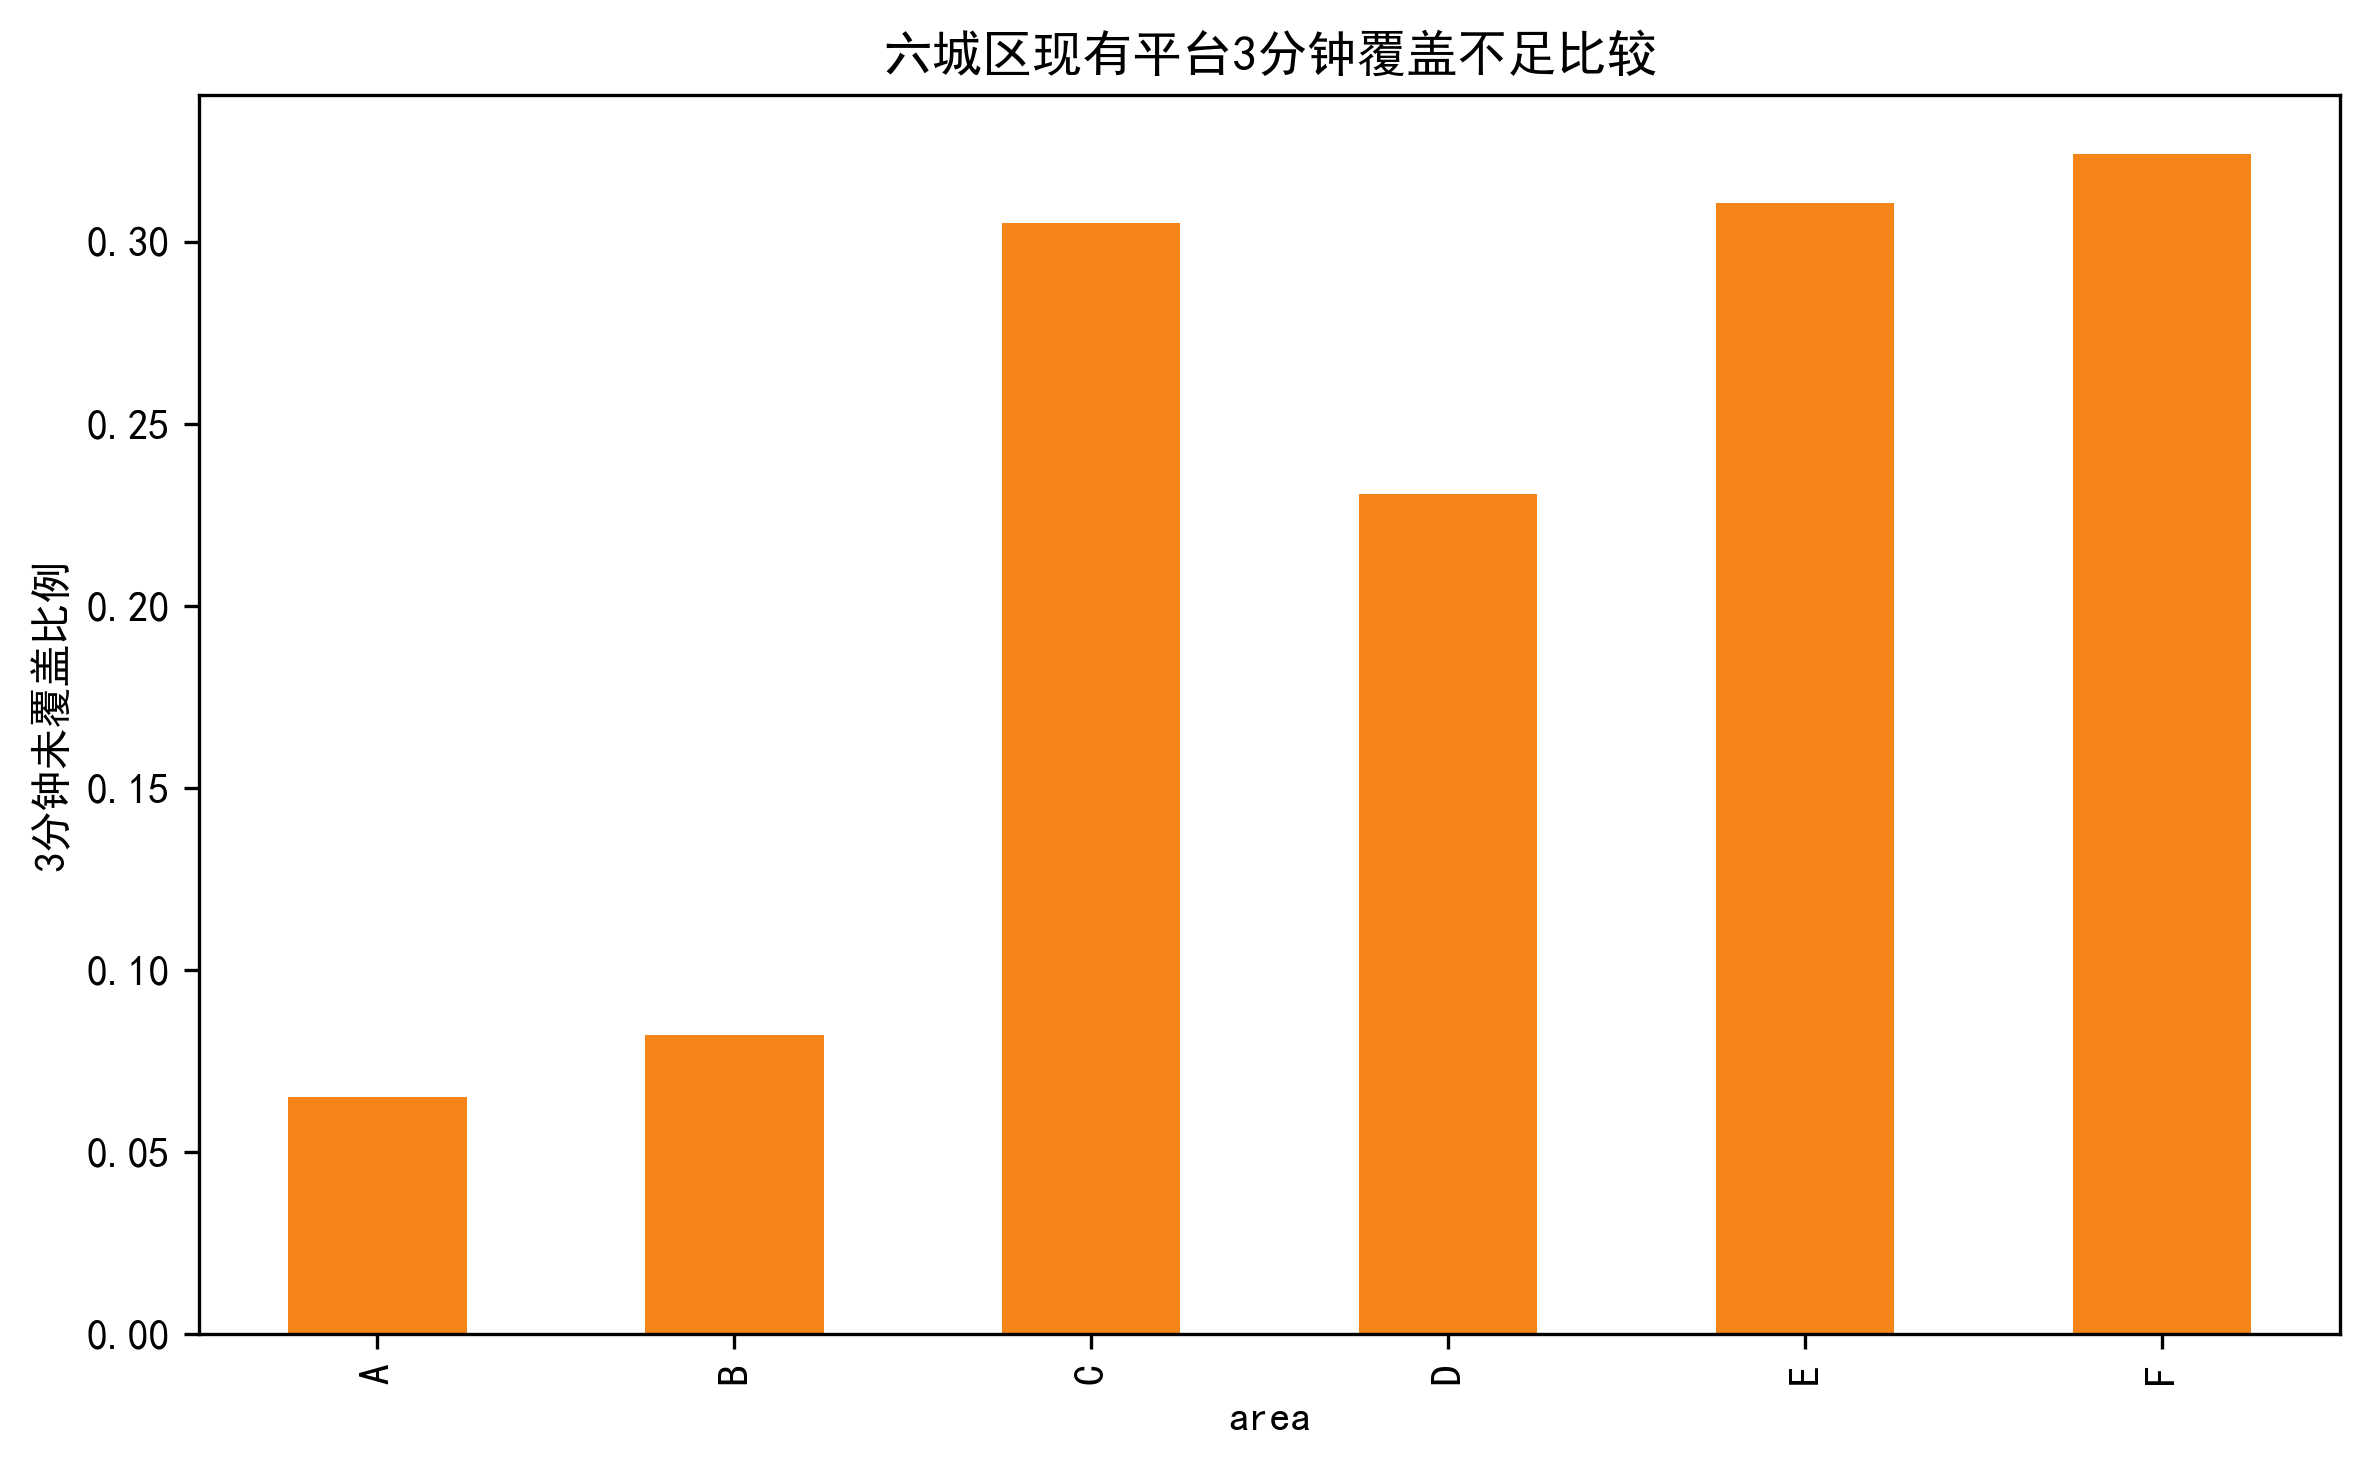
\includegraphics[width=0.82\textwidth]{问题2_六城区覆盖不足率.png}
\caption{六城区现有平台3分钟覆盖不足比较}
\end{figure}
图中可见 C、E、F 等区覆盖不足率明显高于 A、B 区，说明平台资源空间分布与节点规模和路网尺度并不完全匹配。

\begin{figure}[H]\centering
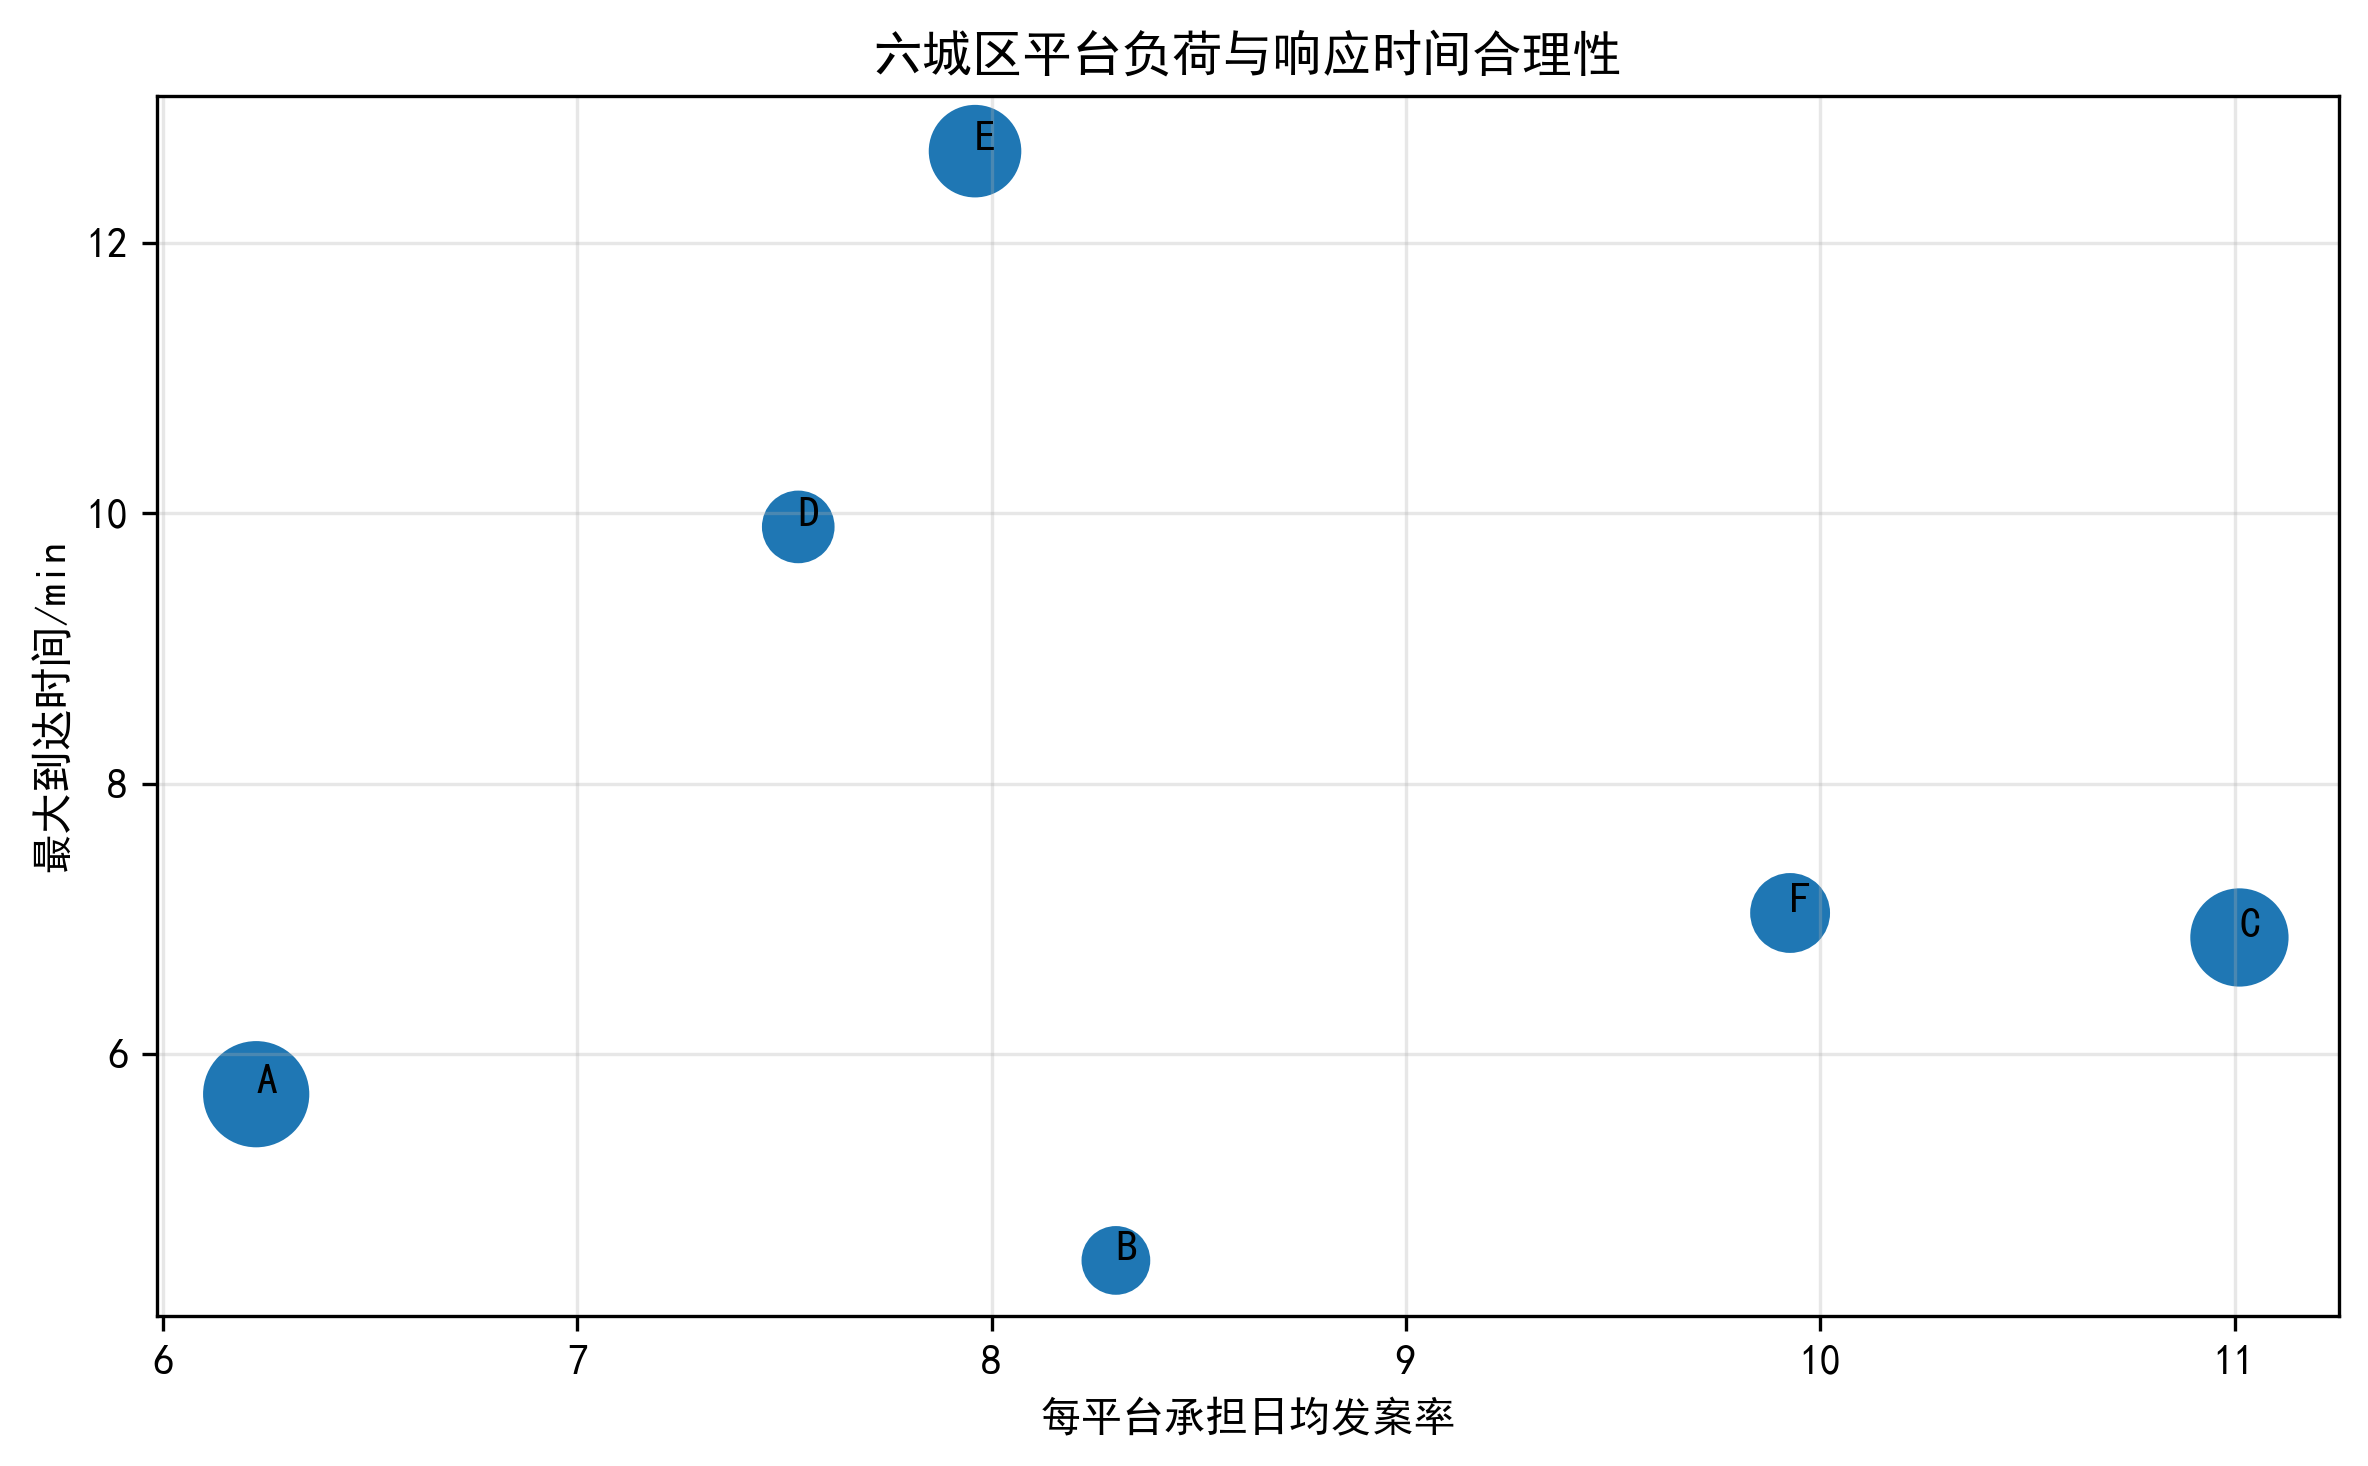
\includegraphics[width=0.82\textwidth]{问题2_六城区合理性散点.png}
\caption{六城区平台负荷与响应时间合理性}
\end{figure}
散点图横轴为每平台承担发案率，纵轴为最大到达时间。位于右上方的城区同时存在工作量高和响应慢问题，应作为优先改进对象。

\subsubsection{改进方案}
为了尽量不改变原有平台体系，本文采用保留 80 个现有平台、逐步新增平台的策略。贪心改进建议新增节点为 517, 315, 408, 455, 206, 392, 509, 285, 239, 261。该方案优先填补远离平台且发案率较高的节点区域；新增后全市未覆盖节点降至 72 个。由于个别远端节点受路网结构限制，单纯少量新增平台仍难以彻底消除所有长响应节点，后续可结合道路等级、平台警力规模和跨区协同进一步优化。

\begin{figure}[H]\centering
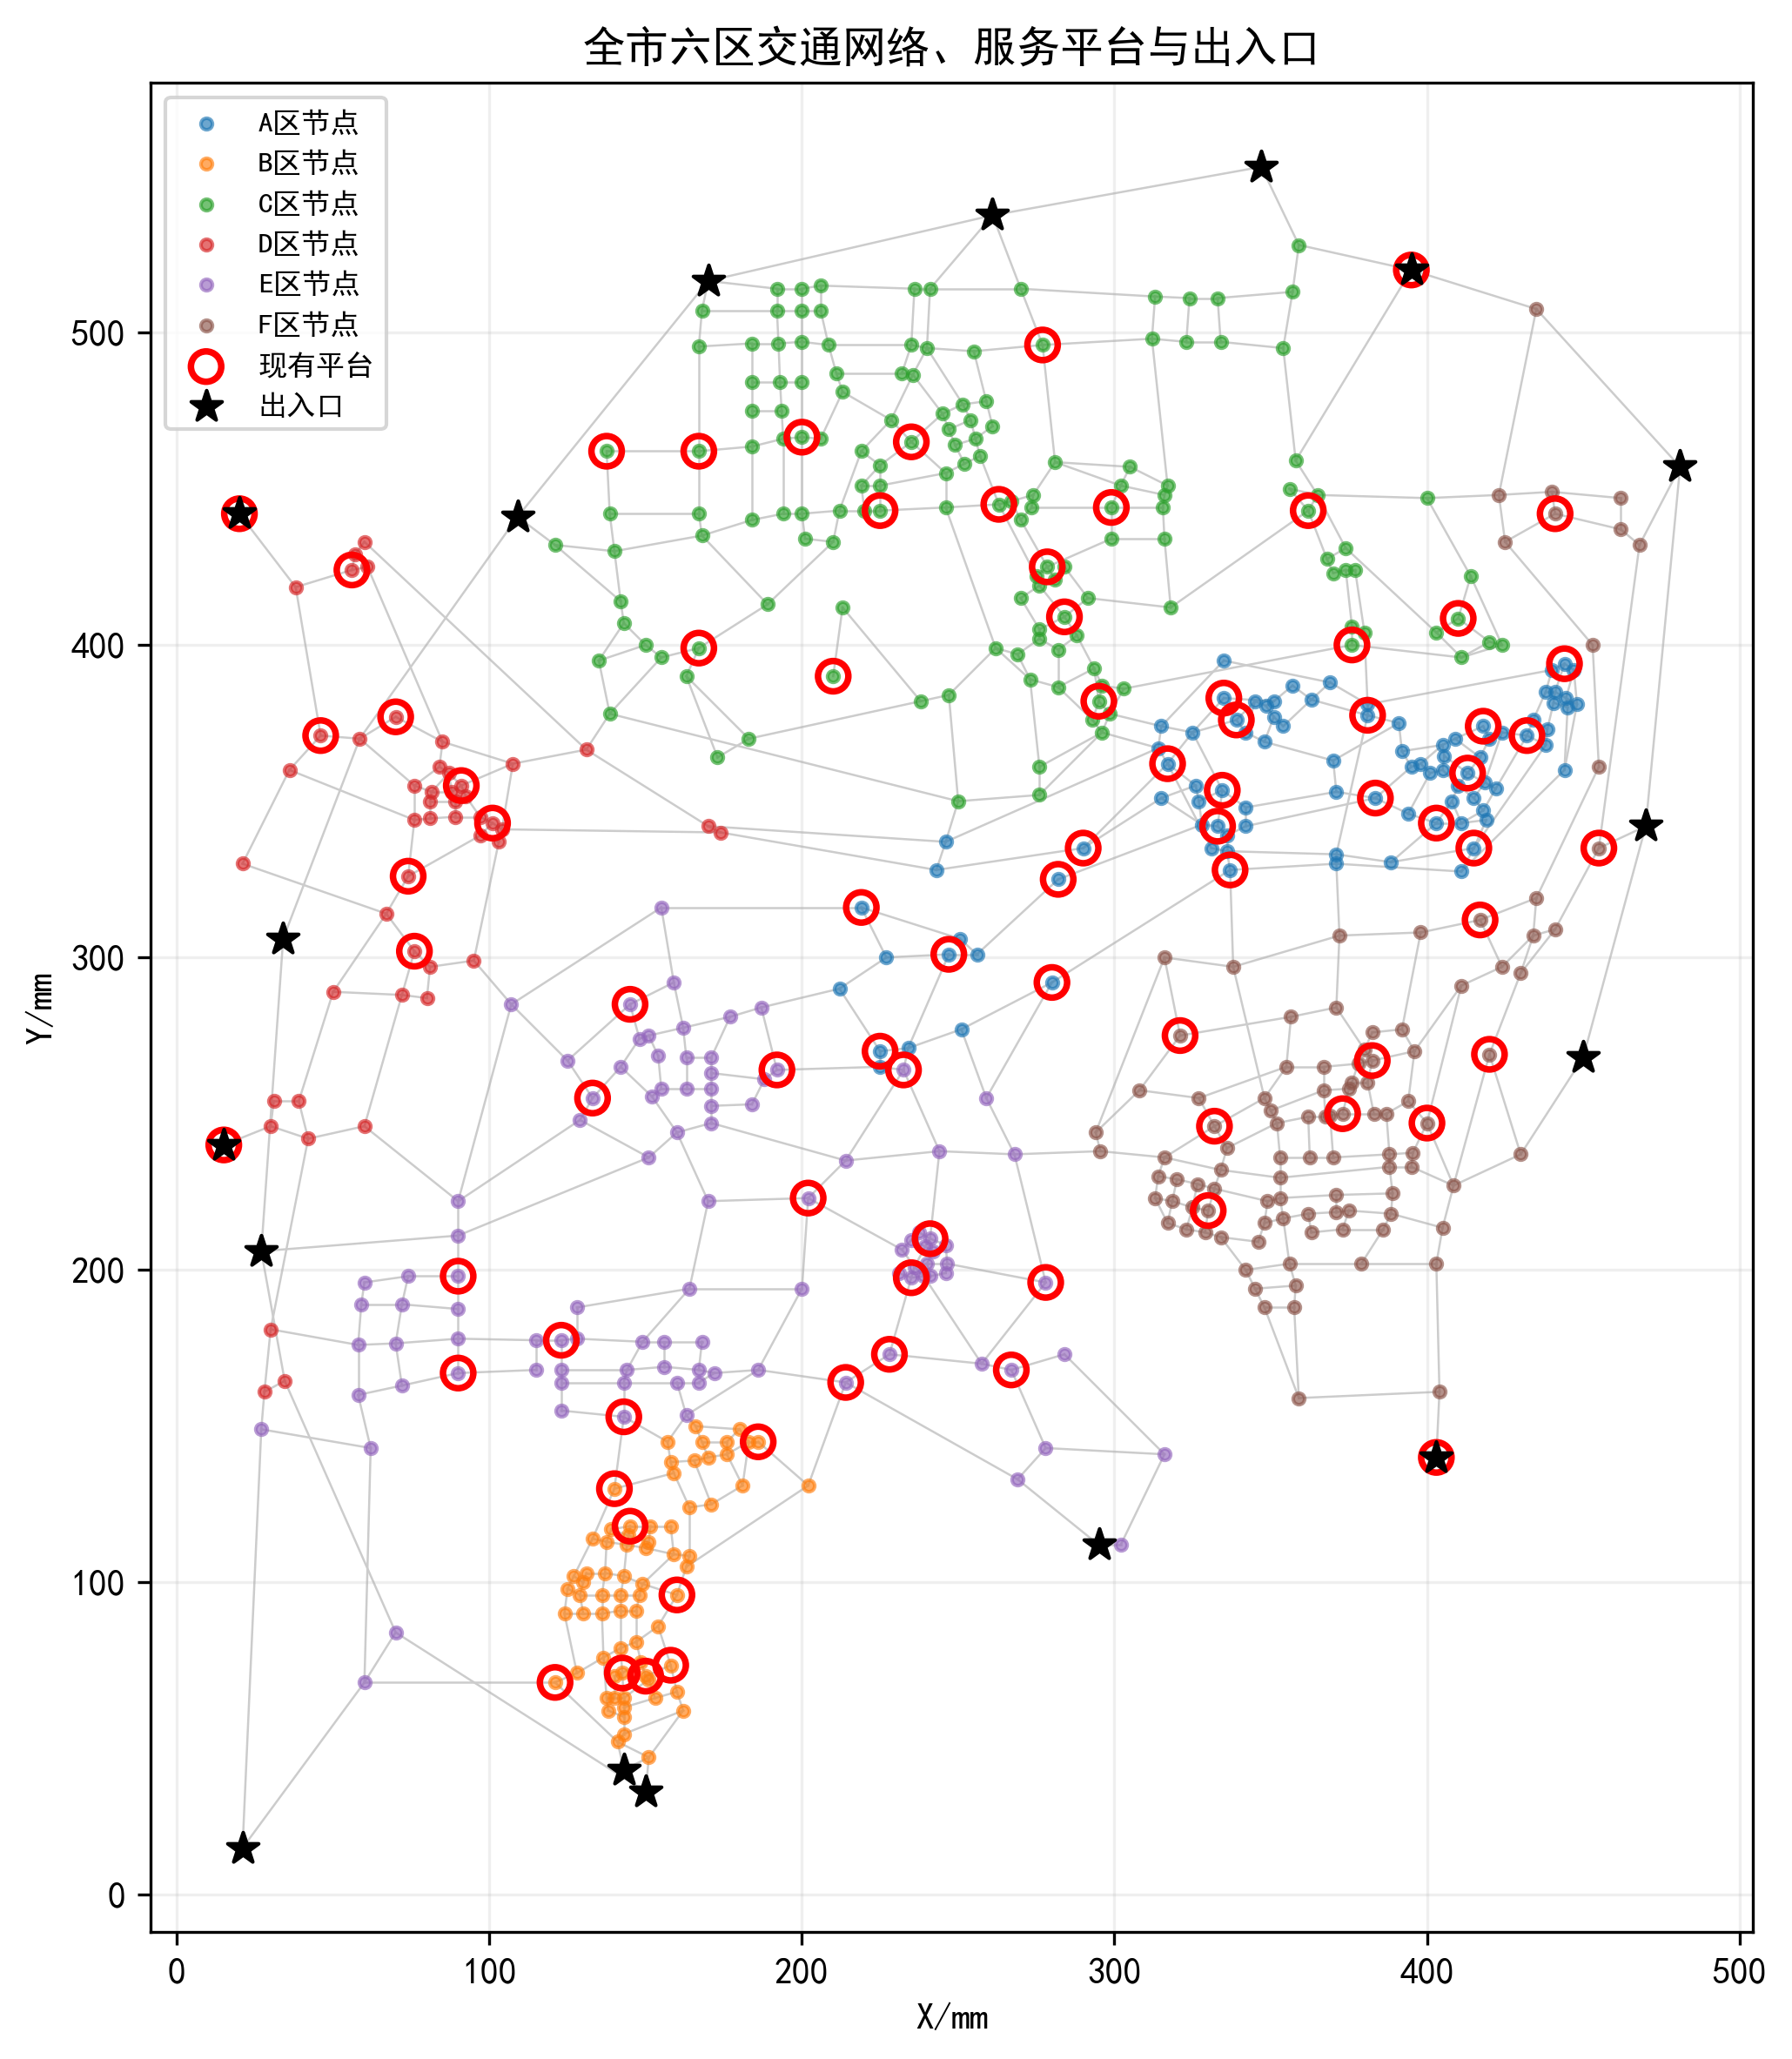
\includegraphics[width=0.82\textwidth]{问题2_全市网络平台与出入口.png}
\caption{全市六区交通网络、服务平台与出入口}
\end{figure}
该图给出了全市路网与平台总体分布。平台并非均匀分布，而是与城区中心和出入口存在较强关联；因此合理性评价不能只看平台数量，还必须结合道路可达性和服务负荷。

\subsection{问题二：P32案发围堵调度}
\subsubsection{模型建立}
设案发点为 $s=32$，报警滞后时间为 $\tau=3$ min。嫌疑人到出口 $e$ 的总最短行驶时间为 $t_s(e)$，报警后剩余时间为
\begin{equation}
R_e=t_s(e)-\tau.
\end{equation}
平台 $p$ 封锁出口 $e$ 的到达时间为 $t(p,e)$。若调度结果满足
\begin{equation}
M_e=R_e-t(p,e)\ge 0,
\end{equation}
则平台可在嫌疑人到达该出口前完成封锁，$M_e$ 称为安全裕度。围堵目标仍采用全市 17 个出入口的瓶颈匹配方案，并检验所有安全裕度是否非负。

\subsubsection{围堵方案与分析}
\begin{table}[H]\centering
\caption{P32案件围堵方案中安全裕度最小的8个出口}
\begin{tabular}{rrrrr}
\toprule
出口 & 平台 & 封锁/min & 嫌疑人剩余/min & 裕度/min \\
\midrule
202 & C10 & 11.620 & 24.879 & 13.259 \\
203 & C13 & 4.448 & 18.824 & 14.377 \\
541 & F10 & 7.042 & 21.860 & 14.818 \\
317 & C16 & 5.475 & 22.152 & 16.677 \\
572 & F11 & 1.655 & 18.746 & 17.091 \\
264 & C1 & 6.622 & 23.966 & 17.344 \\
418 & E8 & 7.419 & 29.231 & 21.812 \\
578 & F5 & 5.758 & 27.813 & 22.056 \\
\bottomrule
\end{tabular}
\end{table}
完整调度表见支撑材料。模型结果表明，所有 17 个出入口均可在嫌疑人到达前完成封锁；最小安全裕度为 13.26 min，风险最高出口为节点 202。该出口应作为指挥中心重点监控点，若现实中存在拥堵、通信延迟或警车速度下降，应优先对该出口派出增援。

\begin{figure}[H]\centering
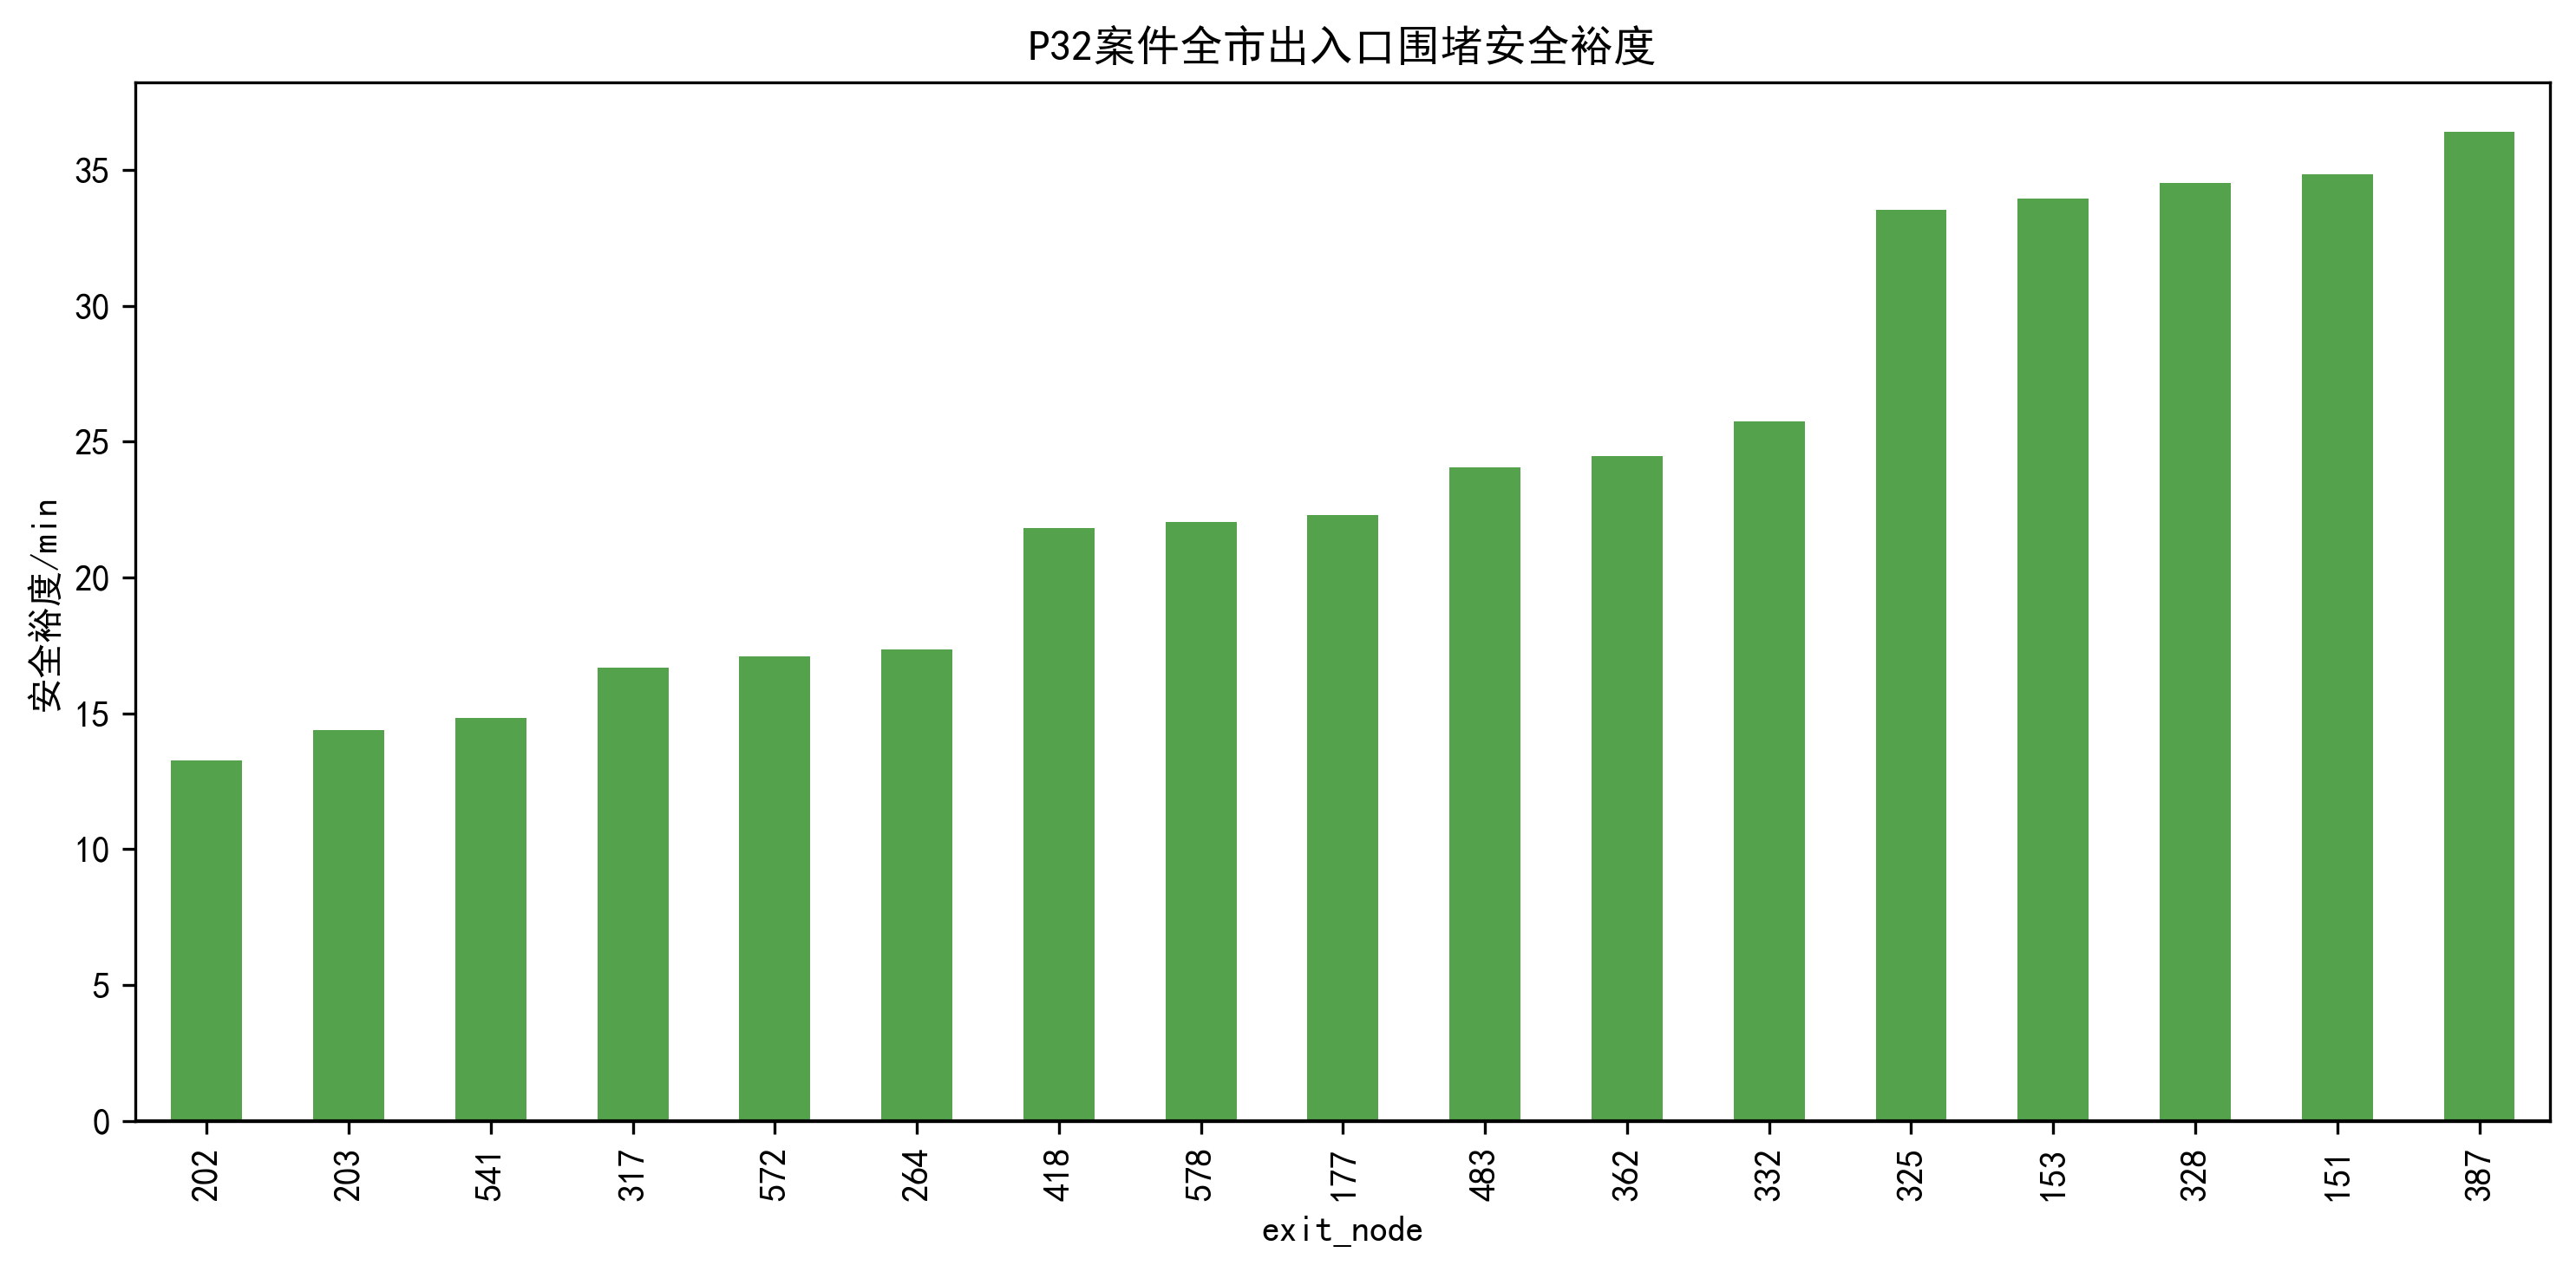
\includegraphics[width=0.82\textwidth]{问题2_P32围堵安全裕度.png}
\caption{P32案件全市出入口围堵安全裕度}
\end{figure}
图中所有柱形均高于 0，说明按本文调度方案，理论上可以在嫌疑人到达所有出入口前完成封控。安全裕度越小的出口越敏感，应在实际指挥中优先确认其警力到位状态。

\section{模型检验、对比与敏感性分析}
\subsection{Baseline 对比}
本文所有核心模型均设置了可解释 baseline。管辖分配的 baseline 是按最近平台分配，主模型进一步用路网最短时间替代简单直线距离，避免道路绕行误判。封锁调度的 baseline 是各出口选择最近平台，但该方法会导致同一平台可能被重复占用；主模型加入“一平台最多封锁一个路口”的匹配约束，更符合题意。新增平台的 baseline 是只增加 2 个平台或只看平均距离；主模型比较 2 至 5 个平台并优先满足 3 min 覆盖约束，因此更贴合题目目标。

\subsection{正确性检验}
数据层面，路网图连通，所有平台与出入口均可达；距离层面，边权由坐标直接计算，时间换算与题目比例一致；优化层面，封锁调度结果中每个出入口恰好对应一个平台，且每个平台最多出现一次，满足题目硬约束。对于 P32 围堵，所有出口安全裕度均非负，说明在模型假设下围堵方案可行。

\subsection{敏感性分析}
对 A 区新增平台数量进行敏感性分析可见，当新增平台数从 2 增加至 4 时，未覆盖节点由 2 降至 0，最大到达时间由 4.19 min 降至 2.90 min；继续增加到 5 个平台时，最大到达时间仅降至 2.71 min。由此可见，新增 4 个平台是覆盖约束的临界点，推荐结论对“是否追求更低平均时间”的偏好有一定敏感性，但对“满足 3 min 约束所需最小平台数”稳定。

对全市评价指标进行扰动分析，若将 3 min 阈值略放宽或收紧，C、E、F 区仍是覆盖不足较突出的区域；若按发案负荷排序，C 区仍为单位平台压力最高区域。因此“全市设置存在不均衡，需要优先改善 C/E/F 等区”的结论稳定。

\section{模型评价、改进与推广}
\subsection{模型优点}
首先，本文直接在道路网络上计算最短路，而不是用直线距离近似，符合警车实际行驶方式。其次，管辖、封锁、选址和围堵问题均以同一套路网距离为基础，保证了不同子问题之间的量纲和逻辑一致。第三，封锁调度采用瓶颈匹配，兼顾重大事件中“最慢出口”这一关键风险。第四，新增平台模型比较 2 至 5 个备选数量，并给出边际收益解释，便于管理部门在资源成本和响应效果之间权衡。

\subsection{模型局限}
本文没有考虑道路拥堵、红绿灯、道路等级、单行线和实际警力数量差异，因此到达时间是理想化平均时间。发案率被视为固定日均强度，未考虑昼夜、节假日和空间相关性变化。新增平台选址采用贪心算法，虽然可解释且稳定，但不能保证在所有组合中全局最优。P32 围堵假设嫌疑人沿最短路径向出入口逃离，现实中嫌疑人可能改变路线或隐藏在城区内部。

\subsection{改进方向}
后续可引入道路实时速度、拥堵概率和道路等级，建立随机旅行时间模型；可根据历史警情时间分布建立分时段平台工作量模型；对新增平台选址可用整数规划或遗传算法搜索全局更优组合；对重大案件围堵可结合动态博弈或最大流最小割思想，不仅封锁出入口，还在关键割点布控，提高对非最短逃逸路径的鲁棒性。

\section{结论}
本文围绕 2011B 交巡警服务平台设置与调度问题，建立了路网最短路、最近服务分配、瓶颈匹配、贪心选址和围堵安全裕度模型。主要结论如下：
\begin{enumerate}[label=(\arabic*)]
  \item A 区现状下有 6 个节点不能 3 min 到达，最大到达时间 5.70 min，平台工作量存在不均衡。
  \item A 区 13 个出入口封锁方案最大到达时间 8.02 min，平均 3.55 min，满足一平台最多封锁一个路口约束。
  \item A 区推荐新增 4 个平台，节点为 28, 40, 48, 87，新增后所有 A 区节点均可在 3 min 内响应。
  \item 全市现状有 138 个节点超过 3 min，F 区覆盖不足最突出，C 区单位平台发案负荷最高，平台设置存在明显不均衡。
  \item P32 案发围堵方案对所有 17 个出入口均可提前封锁，最小安全裕度 13.26 min，风险最高出口为节点 202。
\end{enumerate}

\section{参考文献}
\begin{enumerate}[label={[\arabic*]}]
\item 全国大学生数学建模竞赛组委会. 2011高教社杯全国大学生数学建模竞赛B题及附件[Z]. 2011.
\item Dijkstra E W. A note on two problems in connexion with graphs[J]. Numerische Mathematik, 1959, 1: 269--271.
\item Kuhn H W. The Hungarian method for the assignment problem[J]. Naval Research Logistics Quarterly, 1955, 2(1-2): 83--97.
\item Hakimi S L. Optimum locations of switching centers and the absolute centers and medians of a graph[J]. Operations Research, 1964, 12(3): 450--459.
\item Church R, ReVelle C. The maximal covering location problem[J]. Papers of the Regional Science Association, 1974, 32: 101--118.
\end{enumerate}

\appendix
\section{支撑材料说明}
支撑材料中包含 main\_modeling.py、write\_paper.py、results/frozen\_numbers.json、results/quality\_audit.md、tables 目录下的全部结果表以及 figures 目录下的论文图。所有关键结论均由 main\_modeling.py 一次运行生成，论文数字来自 frozen\_numbers.json 和结果 CSV 表。

\end{document}
